% Overleaf setup: select pdfLaTeX as the compiler.
% Upload this file together with the images and code-listing .txt files
% from the same folder. Compile twice to refresh the contents and lists.
\documentclass[12pt,a4paper,oneside]{report}

% Page layout and fonts
\usepackage[a4paper,margin=1in,headheight=18pt,headsep=10pt,footskip=28pt]{geometry}
\usepackage[T1]{fontenc}
\usepackage[utf8]{inputenc}
\usepackage{lmodern}
\usepackage{setspace}
\usepackage{amsmath,amssymb}

% Tables, figures, lists, and source-code examples
\usepackage{graphicx}
\usepackage{array}
\usepackage{longtable}
\usepackage{tabularx}
\usepackage{enumitem}
\usepackage{float}
\usepackage{xcolor}
\usepackage{listings}

% Headings, page style, and contents/lists formatting
\usepackage{fancyhdr}
\usepackage{titlesec}
\usepackage{tocloft}
\usepackage{caption}

% Diagrams and links
\usepackage{tikz}
\usetikzlibrary{arrows.meta,positioning,shapes.geometric,fit}
\usepackage{url}
\usepackage[hidelinks]{hyperref}

\graphicspath{{./}{figures/}}
\hypersetup{
  pdftitle={AI Forensic Insider Risk Review System},
  pdfauthor={Hrishikesh P S}
}

\newcommand{\projecttitle}{AI Forensic Insider Risk Review System}
\newcommand{\studentname}{HRISHIKESH P S}
\newcommand{\registernumber}{MCA25MCA-2029}
\newcommand{\department}{Department of Computer Applications}
\newcommand{\collegename}{Mar Athanasius College of Engineering}
\newcommand{\collegeplace}{Kothamangalam}
\newcommand{\guide}{Dr.Manu John}
\newcommand{\hod}{Dr.Sonia Abraham}
\newcommand{\degree}{Master of Computer Applications}
\newcommand{\academicyear}{2025--2027}
\newcommand{\collegelogo}[1]{
\includegraphics[width=#1]{logo.png}}

\setlength{\parindent}{0.35in}
\setlength{\parskip}{0.25em}
\setlength{\tabcolsep}{5pt}
\renewcommand{\arraystretch}{1.2}
\setcounter{secnumdepth}{3}
\setcounter{tocdepth}{3}
\setlength{\cftsecnumwidth}{3.2em}
\setlength{\cftsubsecnumwidth}{4.2em}
\setlength{\cftsubsubsecnumwidth}{5.2em}
\setlist[itemize]{leftmargin=1.5em,itemsep=0.25em,topsep=0.35em}
\setlist[enumerate]{leftmargin=1.7em,itemsep=0.3em,topsep=0.35em}
\setlength{\emergencystretch}{3em}

\titleformat{\chapter}[hang]
  {\bfseries\fontsize{16}{20}\selectfont}
  {\thechapter.}{0.65em}{}
\titlespacing*{\chapter}{0pt}{-8pt}{18pt}
\titleformat{\section}[hang]
  {\bfseries\fontsize{14}{18}\selectfont}
  {\thesection}{0.7em}{}
\titlespacing*{\section}{0pt}{16pt}{7pt}
\titleformat{\subsection}[hang]
  {\bfseries\fontsize{12}{15}\selectfont}
  {\thesubsection}{0.7em}{}
\titlespacing*{\subsection}{0pt}{12pt}{5pt}
\titleformat{\subsubsection}[hang]
  {\bfseries\fontsize{12}{14}\selectfont}
  {\thesubsubsection}{0.7em}{}
\titlespacing*{\subsubsection}{0pt}{10pt}{4pt}

\fancypagestyle{reportstyle}{
  \fancyhf{}
  \fancyhead[R]{\small\projecttitle}
  \fancyfoot[L]{\small\department}
  \fancyfoot[R]{\thepage}
  \renewcommand{\headrulewidth}{0.4pt}
  \renewcommand{\footrulewidth}{0.4pt}
}
\fancypagestyle{plain}{
  \fancyhf{}
  \fancyhead[R]{\small\projecttitle}
  \fancyfoot[L]{\small\department}
  \fancyfoot[R]{\thepage}
  \renewcommand{\headrulewidth}{0.4pt}
  \renewcommand{\footrulewidth}{0.4pt}
}

\definecolor{codegray}{gray}{0.94}
\definecolor{rulegray}{gray}{0.45}
\lstset{
  basicstyle=\ttfamily\scriptsize,
  numbers=left,
  numberstyle=\tiny\color{gray},
  numbersep=7pt,
  frame=single,
  rulecolor=\color{rulegray},
  backgroundcolor=\color{codegray},
  breaklines=true,
  breakatwhitespace=false,
  keepspaces=true,
  showstringspaces=false,
  tabsize=4,
  columns=fullflexible,
  captionpos=b,
  literate={·}{{.}}1 {×}{{x}}1 {–}{{--}}1 {—}{{---}}1
    {’}{{'}}1 {“}{{``}}1 {”}{{''}}1 {…}{{...}}1
    {→}{{->}}1 {↗}{{$\nearrow$}}1 {⌁}{{~}}1 {⌂}{{H}}1 {⌕}{{?}}1
    {▦}{{[grid]}}1 {▧}{{[folder]}}1 {◇}1 {◈}1
    {◉}{{(o)}}1 {◎}{{( )}}1 {♙}{{P}}1 {✦}{{*}}1 {✳}{{+}}1
    {＋}{{+}}1
}

\newcolumntype{Y}{>{\raggedright\arraybackslash}X}
\newcolumntype{R}{>{\raggedleft\arraybackslash}X}
\newcommand{\tablefont}{\small}
\newcommand{\code}[1]{\texttt{\small #1}}

% Keep the numbered References chapter without the report class's second heading.
\makeatletter
\renewenvironment{thebibliography}[1]
  {\list{\@biblabel{\@arabic\c@enumiv}}%
       {\settowidth\labelwidth{\@biblabel{#1}}%
        \leftmargin\labelwidth
        \advance\leftmargin\labelsep
        \@openbib@code
        \usecounter{enumiv}%
        \let\p@enumiv\@empty
        \renewcommand\theenumiv{\@arabic\c@enumiv}}%
   \sloppy
   \clubpenalty4000
   \@clubpenalty\clubpenalty
   \widowpenalty4000%
   \sfcode`\.\@m}
  {\def\@noitemerr
       {\@latex@warning{Empty `thebibliography' environment}}%
   \endlist}
\makeatother

\begin{document}
% Title and certificate pages are omitted as requested.
\pagenumbering{roman}
\fancypagestyle{frontmatter}{\fancyhf{}\fancyfoot[C]{\textit{\thepage}}\renewcommand{\headrulewidth}{0pt}\renewcommand{\footrulewidth}{0pt}}
\fancypagestyle{plain}{\fancyhf{}\fancyfoot[C]{\textit{\thepage}}\renewcommand{\headrulewidth}{0pt}\renewcommand{\footrulewidth}{0pt}}
\renewcommand{\cftlottitlefont}{\hfill\bfseries\fontsize{16}{20}\selectfont}\renewcommand{\cftafterlottitle}{\hfill}
\renewcommand{\cftloftitlefont}{\hfill\bfseries\fontsize{16}{20}\selectfont}\renewcommand{\cftafterloftitle}{\hfill}
\pagestyle{frontmatter}
\titleformat{\chapter}[block]{\bfseries\fontsize{16}{20}\selectfont\centering}{}{0pt}{}
\renewcommand{\cfttoctitlefont}{\hfill\bfseries\fontsize{16}{20}\selectfont}\renewcommand{\cftaftertoctitle}{\hfill}

\chapter*{Acknowledgement}
\addcontentsline{toc}{chapter}{Acknowledgement}
I express my sincere gratitude to the management of Mar Athanasius
College of Engineering, Kothamangalam, for providing the academic
environment and facilities needed to undertake this mini project. The
project gave me an opportunity to apply my learning in data science,
machine learning, software development, and responsible data analysis.

I extend my heartfelt appreciation to my project guide, Dr.Manu John,
Department of Computer Applications, for his valuable guidance,
technical suggestions, and encouragement throughout the planning,
development, and documentation of the AI Forensic Insider Risk Review
System. His feedback helped me refine the project and present its
methods and limitations more clearly.

I am sincerely grateful to Dr.Sonia Abraham, Head of the Department of
Computer Applications, for her encouragement and support. I also thank
the project coordinators, faculty members, and staff of the department
for their guidance and assistance during the project.

I acknowledge the creators of the CERT Insider Threat Test Dataset and
the developers and maintainers of the open-source tools used in this
work. Their contributions supported the study of synthetic activity
records and the implementation of the data-processing, modelling, and
dashboard components.

Finally, I express my heartfelt gratitude to my parents, family
members, and friends for their patience, encouragement, and support. I
also thank everyone who contributed directly or indirectly to the
completion of this mini project and its report.

\chapter*{Abstract}
\addcontentsline{toc}{chapter}{Abstract}
Insider-risk review is difficult because potentially relevant activity
is distributed across multiple systems, the number of routine events is
large, and known incident examples are rare. This mini project presents
Forensio, a local-first review system that aggregates logon, removable
device, file, email, and web activity into employee-day features and
uses four different model perspectives to prioritize records for human
inspection. The implementation combines a Python data and scoring
pipeline, a FastAPI service, and a React review dashboard; a Streamlit
interface remains available as an alternative.

The model-development study uses the CERT r4.2 synthetic insider-threat
dataset. Its saved labelled table contains 330,452 employee-days for
1,000 synthetic users, of which 1,364 employee-days overlap a listed
incident interval under the project's labeling rule. Activity events
are cleaned and aggregated by user and calendar day. A grouped
train/validation/test design keeps users disjoint between partitions.
The notebook compares Logistic Regression, Decision Tree, Random
Forest, and Isolation Forest, selects variants and a review capacity
using validation data, and evaluates the selected operating point on a
held-out test partition. In the saved one-percent review-capacity
evaluation, the Random Forest has precision 0.144, recall 0.329, F1
0.200, and average precision 0.158. The dashboard separately combines
within-dataset percentile ranks and applies an employee-level queue
rule.

The system is a research and demonstration prototype, not an
investigative finding engine. A high rank is neither a probability nor
evidence of misconduct. The dataset is synthetic, labels are
incident-window proxies, queue rules are relative to a selected
dataset, and the current features do not model employee roles,
schedules, or context. Human review, corroborating evidence, access
controls, and documented governance are therefore essential before any
operational use.

\renewcommand{\listtablename}{List of tables}
\listoftables

\renewcommand{\listfigurename}{List of figures}
\listoffigures

\clearpage
\pagestyle{frontmatter}
\tableofcontents

\clearpage
\pagenumbering{arabic}
\setcounter{page}{1}
\titleformat{\chapter}[hang]{\bfseries\fontsize{16}{20}\selectfont}{\thechapter.}{0.65em}{}
\fancypagestyle{plain}{\fancyhf{}\fancyhead[R]{\small\projecttitle}\fancyfoot[L]{\small\department}\fancyfoot[R]{\thepage}\renewcommand{\headrulewidth}{0.4pt}\renewcommand{\footrulewidth}{0.4pt}}
\pagestyle{reportstyle}
\onehalfspacing

\chapter{Introduction}
\label{chap:introduction}

\section{Background}
Modern organisations generate activity records through identity
providers, endpoints, file services, email systems, and web gateways.
These records are useful for security operations, but their volume and
fragmentation make manual review difficult. A security analyst may
need to correlate a sequence of events across several sources before
deciding whether it warrants escalation. The challenge is not simply
to detect a single unusual event; it is to organise context in a way
that supports a careful and reproducible investigation.

Insider-risk analysis concerns activity associated with trusted
accounts and authorised access. A meaningful review must distinguish
between a statistical signal and a conclusion about a person.
Legitimate work can produce unusual activity, while harmful activity
may resemble normal operations. Differences in job role, work schedule,
travel, project deadlines, and system configuration can all affect the
observed event pattern. For that reason, a decision-support tool should
make its inputs and ranking logic understandable and should preserve
human authority over all consequential decisions.

This project implements a prototype called Forensio. It transforms
five activity logs into employee-day counts, scores those feature rows
using four model families, and displays a ranked review queue. It is
designed to demonstrate a technical workflow on the CERT r4.2
synthetic dataset. It is not a production surveillance platform, does
not inspect message or file content, and does not establish intent.

\section{Problem statement}
The project addresses the following bounded problem: given a local
folder containing the five supported activity CSV files and a
previously trained model bundle, produce an employee-day and
employee-level ranking that helps an analyst decide which records to
review first. The system must integrate disparate sources, handle
large CSV files with bounded-memory processing, apply the same feature
contract used in training, expose clear model context, and avoid
presenting a score as proof.

The study also evaluates whether a set of supervised and unsupervised
models can rank synthetic incident-window employee-days above other
days when users are kept separate across development and test
partitions. A low base rate makes accuracy alone unsuitable as the
primary measure. The study therefore reports average precision and
capacity-based precision, recall, and F1 alongside the confusion
counts.

\section{Objectives of the project}
The objectives are to:
\begin{enumerate}
  \item examine the supported activity data and its quality;
  \item build a repeatable employee-day aggregation and labeling
  workflow;
  \item compare four distinct model families under user-grouped
  evaluation;
  \item build a local scoring service that reuses the trained feature
  schema;
  \item create a dashboard for selecting data, following analysis
  progress, and reviewing ranked employees and activity details;
  \item document evaluation limits, privacy considerations, and
  responsible-use controls.
\end{enumerate}

\section{Scope of the project}
The project scope includes synthetic logon, device, file, email, and
HTTP event records; aggregation at one calendar day per user; the
feature columns persisted with the trained bundle; offline model
evaluation; local scoring; and a human-readable review interface.
Optional employee-name lookup files are supported by the local scoring
code, but names are not required for model input.

The current scope excludes live collection agents, enterprise identity
integrations, cross-organisation model transfer, streaming analysis,
automated disciplinary decisions, legal attribution, message-body or
file-content inspection, calibrated probability estimates, and
production authentication or role-based access control. A dashboard
rank is relative to the data batch being scored. The offline
employee-day test results do not validate the dashboard's
employee-level status rule.

\section{Project domain and technology stack}
The project combines data engineering, applied machine learning,
information visualization, and digital-forensics workflow concepts.
Python and pandas perform input handling and aggregation;
scikit-learn supplies estimators and metrics; joblib persists the
model bundle; FastAPI exposes a local HTTP interface; and React,
JavaScript, Vite, and CSS provide the browser dashboard. Streamlit is
retained as an alternative interface. CSV files are used for both
inputs and result exports; the prototype does not require a database.

\begin{table}[H]
\centering
\tablefont
\caption{Project components and their responsibilities}
\label{tab:technology-stack}
\begin{tabularx}{\textwidth}{|p{0.24\textwidth}|p{0.25\textwidth}|Y|}
\hline
\textbf{Component} & \textbf{Technology} & \textbf{Responsibility}\\\hline
Data preparation & Python, pandas, NumPy & Clean activity records, aggregate features, and align model columns.\\\hline
Model development & scikit-learn & Fit and evaluate supervised and unsupervised estimators.\\\hline
Model persistence & joblib & Store estimators and the feature-column contract for local reuse.\\\hline
Service layer & FastAPI, Pydantic & Validate requests, manage analysis endpoints, and return JSON results.\\\hline
Web interface & React, Vite, CSS & Select log folders, display progress, search and filter the review queue.\\\hline
Alternative interface & Streamlit & Provide a Python-only local demonstration path.\\\hline
Input and outputs & CSV & Interchange activity logs, scores, and report tables.\\\hline
\end{tabularx}
\end{table}

\section{Organisation of the report}
Chapter 2 reviews insider-risk analytics and relevant evaluation
principles. Chapter 3 describes the dataset, preprocessing,
visualization, algorithms, pipeline, feasibility, and operating
environment. Chapter 4 presents model construction, software
architecture, requirements, data design, and interface design.
Chapter 5 reports the saved model evaluation and discusses its limits.
Chapter 6 describes the local deployment and analyst workflow.
Chapter 7 summarises the repository history. Chapters 8 and 9 give the
conclusions and future work. Chapter 10 contains reproducibility
information, requirements, test cases, data definitions, responsible
use guidance, and source listings. Chapter 11 provides references.

\chapter{Supporting literature}
\label{chap:literature}

\section{Literature review}
Insider-risk detection is difficult because legitimate and risky
activities can share the same systems and permissions. Research
therefore examines both user behaviour and the context needed to
interpret it, rather than treating a model score as proof of intent.
The CERT Insider Threat Test Dataset provides synthetic scenarios and
activity records for repeatable experiments \cite{cert}. Synthetic
data avoids exposing real employee records during development, but
results on one generated release do not establish performance in a
real organisation.

Rahman, Al Naeem, and Abubakar study unintentional-insider readiness
using CERT r4.2 activity data and a nonlinear autoregressive model with
exogenous inputs (NARX). They describe access, motivation, and action
as dimensions of insider behaviour and report a best-partition
\(R^2\) value of 0.97 for their proposed formulation
\cite{rahman2022unintentional}. This work is relevant because it
explicitly considers unintentional rather than exclusively malicious
behaviour. Its target formulation and reported statistic differ from
the employee-day classification and review-capacity metrics used in
this project, so the figures should not be compared as if they measured
the same task.

Al-Shehari et al. investigate an anomaly-based Isolation Forest model
for the class-imbalance problem in insider-threat data, using the CERT
benchmark and varying the model's contamination setting. They report
98\% accuracy for their proposed approach
\cite{alshehari2023isolation}. The study motivates including an
unsupervised anomaly detector alongside supervised classifiers.
However, accuracy alone does not describe how many rare positive cases
are found or how many reviewed records are positive. For an imbalanced
review queue, precision, recall, average precision, and results at a
specified review capacity provide additional information.

Insider-risk prioritisation is related to, but distinct from,
digital-forensics-based attack detection. Dimitriadis et al. present
Fronesis, which correlates digital artifacts with MITRE ATT\&CK
techniques and Cyber Kill Chain phases using an ontology and
rule-based reasoning; they demonstrate the approach with a phishing
scenario \cite{dimitriadis2023fronesis}. This work highlights the
importance of preserving and correlating evidence. The present project
has a narrower analytical scope: it ranks synthetic employee-day
records and directs a reviewer to source activity, rather than
detecting an ongoing attack or reconstructing a forensic timeline.

The project follows a common feature-engineering pattern: transform
event-level data into a table whose rows represent a user and a
calendar day. Aggregation reduces the number of records and makes
multi-source activity easier to compare. Count and timing features can
reveal volume changes or activity outside a fixed interval, but they
lose event ordering and detailed context. A day-level table cannot
reconstruct a forensic timeline. The system therefore treats the
aggregate as a navigation aid and directs an analyst back to original
records for validation.

The algorithm set deliberately includes contrasting assumptions.
Logistic Regression is a linear supervised classifier and provides a
relatively simple baseline. A Decision Tree expresses threshold
relationships through a sequence of splits but can overfit if
unconstrained. A Random Forest averages many trees to reduce the
instability of a single tree. Isolation Forest isolates observations
through random feature and split selection, assigning higher anomaly
scores to observations isolated in fewer splits
\cite{liu2008isolation}. The estimator used in this project is
implemented by scikit-learn \cite{sklearn}. These algorithms do not
produce interchangeable quantities: a class probability, a decision
function, and an anomaly score have different semantics. This project
converts each output to a percentile rank within the current scoring
batch before combining dashboard scores.

Rare labels and high class imbalance are central evaluation concerns.
When a positive example is a small fraction of a test set, a model can
achieve high accuracy by ranking nearly all records as negative.
Precision-recall measures are more informative for a review queue
because they describe the fraction of selected records matching known
positive labels and the fraction of known positives retrieved. Average
Precision summarises precision over score thresholds. A fixed-capacity
queue also corresponds to an operational constraint: an analyst can
review only a limited number of records in a given period. Evaluation
must specify whether capacity selection was performed on validation
data or the test set.

User-level leakage is another important issue in behavioural data.
Repeated daily records from one person share stable characteristics.
If records are randomly distributed across training and testing, the
model may benefit from seeing a user's other days before evaluation.
The notebook therefore uses stratified group splitting with the user
identifier as the group. The identifier is not a model feature; it is
used to keep users in one partition.

Responsible monitoring practices require a clear purpose, access
limits, proportionality, retention controls, and a review process.
Security frameworks such as NIST SP 800-53 describe system and
information security controls, while NIST SP 800-61 describes incident
response practices \cite{nist53,nist61}. These documents are not
specific model-governance standards, but they provide useful control
contexts for access, logging, incident handling, and evidence
preservation. A risk score alone should not trigger an adverse action.

\section{Literature review summary}
\begin{table}[H]
\centering
\tablefont
\caption{Literature themes and their application to this project}
\label{tab:literature-themes}
\begin{tabularx}{\textwidth}{|p{0.24\textwidth}|p{0.34\textwidth}|Y|}
\hline
\textbf{Theme} & \textbf{Practical implication} & \textbf{Project response}\\\hline
Synthetic and unintentional-insider research & CERT supports repeatable experiments; the unintentional-insider study uses a different target formulation. & Use CERT r4.2 and limit conclusions to this project's employee-day labels and evaluation protocol.\\\hline
Anomaly detection under class imbalance & Isolation Forest offers a label-independent scoring perspective; accuracy alone may hide minority-class performance. & Compare it with supervised models using ranking and fixed-capacity metrics.\\\hline
Digital-forensics-based detection & Correlating artifacts with attack techniques can support incident detection and evidence interpretation. & Treat the dashboard as a prioritisation aid and require analyst validation against original records.\\\hline
Event aggregation & Simplifies modelling but removes sequence and context. & Aggregate to employee-day counts and preserve source records for follow-up.\\\hline
Rare positive labels & Accuracy can conceal low precision and missed cases. & Report AP and capacity-based precision, recall, F1, and confusion counts.\\\hline
Repeated observations & Random row splits can leak individual patterns. & Keep employees disjoint across training, validation, and test partitions.\\\hline
Human investigation & A ranking or a detected artifact is not, by itself, a finding about intent or misconduct. & Display review language and require independent analyst verification.\\\hline
\end{tabularx}
\end{table}

\section{Findings and proposals}
The reviewed papers address complementary problems: unintentional
insider readiness, anomaly scoring under class imbalance, and
forensics-based correlation of evidence during an ongoing attack.
Their targets, methods, and reported metrics differ, so their
published results are context rather than a direct benchmark for this
implementation. Together with the CERT dataset documentation, they
motivate four design decisions. First, the project uses a multi-source
daily representation rather than treating each event as an independent
case. Second, it compares model families instead of presuming that one
algorithm is universally suitable. Third, it separates model selection
from final test reporting and reports review-capacity metrics for rare
labels. Fourth, it describes the interface as a review aid and makes
the relative nature of the scores explicit.

The literature also identifies gaps that remain open. A future
evaluation should include time-based testing, additional synthetic
releases, calibrated and subgroup-aware analyses where ethically and
lawfully appropriate, and structured analyst feedback. Before any
real-world use, an organisation would need to define a lawful purpose,
consult relevant stakeholders, assess privacy and employment impacts,
set retention limits, control access, and validate the complete
workflow rather than only the estimator.

\chapter{System analysis}
\label{chap:analysis}

\section{Analysis of the dataset}

\subsection{About the dataset}
The development notebook reads the CERT r4.2 release from the
repository's local \code{r4.2} folder and the matching
\code{answers/insiders.csv} answer file. The activity sources are
\code{logon.csv}, \code{device.csv}, \code{file.csv},
\code{email.csv}, and \code{http.csv}. The answer file is used during
offline training and evaluation; a dashboard user supplies activity
logs only. It is not a live incident feed.

\begin{table}[H]
\centering
\tablefont
\caption{Activity-source inventory and the information used}
\label{tab:source-inventory}
\begin{tabularx}{\textwidth}{|p{0.22\textwidth}|p{0.24\textwidth}|Y|}
\hline
\textbf{Source} & \textbf{Role in the pipeline} & \textbf{Aggregated information}\\\hline
\code{logon.csv} & Authentication activity & Event count and count before 06:00 or at/after 18:00.\\\hline
\code{device.csv} & Removable-device activity & Event count, after-hours count, and connect-event count.\\\hline
\code{file.csv} & File-system activity & Event count and after-hours count; file contents are not read.\\\hline
\code{email.csv} & Email activity & Event count, after-hours count, and numeric attachment total.\\\hline
\code{http.csv} & Web activity & Event count and after-hours count; URL content is not modelled.\\\hline
\code{answers/\allowbreak insiders.csv} & Research labels & User, incident interval, scenario, and dataset version for offline labels.\\\hline
\end{tabularx}
\end{table}

The saved labelled employee-day table contains 330,452 rows for 1,000
synthetic users. Its calendar coverage runs from 2 January 2010 through
17 May 2011. The project labeling rule marks 1,364 employee-days as
positive, or approximately 0.413 percent. The positive days belong to
70 user identifiers. These values describe the saved project
artifacts; they are not estimates of prevalence in a real workforce.

\subsection{Explore the dataset}
The five source files contain 32,770,222 raw event rows in total.
The recorded cleaning summary retains 32,409,354 rows and removes
360,868 duplicate rows. No missing user identifiers or invalid dates
are reported in those saved summaries. Most records are in the HTTP
source, so a single source can dominate an event-volume plot. The
features used by the model are counts, not concatenated raw event
histories.

\begin{table}[H]
\centering
\tablefont
\caption{Saved data-cleaning summary}
\label{tab:cleaning-summary}
\begin{tabularx}{\textwidth}{|p{0.22\textwidth}|R|R|R|R|}
\hline
\textbf{Source} & \textbf{Rows read} & \textbf{Rows kept} & \textbf{Duplicates removed} & \textbf{Rows dropped}\\\hline
Logon & 854,859 & 854,859 & 0 & 0\\\hline
Device & 405,380 & 405,374 & 6 & 6\\\hline
File & 445,581 & 445,581 & 0 & 0\\\hline
Email & 2,629,979 & 2,618,056 & 11,923 & 11,923\\\hline
HTTP & 28,434,423 & 28,085,484 & 348,939 & 348,939\\\hline
\textbf{Total} & \textbf{32,770,222} & \textbf{32,409,354} & \textbf{360,868} & \textbf{360,868}\\\hline
\end{tabularx}
\end{table}

The cleaning report counts duplicate removals within the implemented
chunk-processing workflow. Deduplication performed independently
inside separate chunks may not remove a duplicate whose copies fall in
different chunks. Therefore, the saved counts should be interpreted
according to the implementation rather than as proof of global,
cross-chunk uniqueness. If global deduplication is required, the
pipeline should be extended and its memory and identity semantics
specified.

\subsection{Dataset limitations}
CERT r4.2 is a synthetic benchmark. Its events, scenarios, identities,
and incident windows are useful for repeatable experiments but do not
represent a verified real employee population. There is no guarantee
that the synthetic incident patterns cover all plausible behaviours,
that background distributions match another organisation, or that a
trained score will generalise across job roles and time periods.

The five activity tables are not necessarily complete observations of
all employee behaviour. Missing sources, source-specific collection
gaps, clock differences, account-sharing, and system changes can all
alter counts. The prototype currently assumes that timestamps can be
parsed and converted into a calendar day without a configured
organisation-specific time zone. These assumptions should be checked
before a different dataset is analysed.

\section{Data preprocessing}

\subsection{Data cleaning}
The production scoring core reads each CSV in chunks of 25,000 rows.
Column names are normalised to lower case and stripped of surrounding
spaces. The parser requires usable \code{date} and \code{user}
columns, trims user identifiers, parses dates with invalid values
coerced to missing, removes rows with unusable users or dates, and
deduplicates rows within a chunk. It then derives a calendar-day key,
an after-hours indicator, and any source-specific features. Each
source is grouped on user and day before source tables are combined.

After-hours activity is defined mechanically as an event before 06:00
or at/after 18:00. The boundary is inclusive at 18:00. This fixed
interval is not adjusted for shifts, daylight-saving interpretation,
holidays, travel, or personal schedules. It is a research feature, not
a policy determination.

\begin{table}[H]
\centering
\tablefont
\caption{Preprocessing decisions and their consequences}
\label{tab:preprocessing-decisions}
\begin{tabularx}{\textwidth}{|p{0.24\textwidth}|p{0.38\textwidth}|Y|}
\hline
\textbf{Decision} & \textbf{Implementation behaviour} & \textbf{Consequence to consider}\\\hline
Chunked ingestion & Reads up to 25,000 records per chunk. & Bounds the size of an individual read but does not make all later tables constant-memory.\\\hline
Header normalisation & Trims and lowercases selected field names. & Helps tolerate case and whitespace differences; schema aliases remain limited.\\\hline
Timestamp parsing & Invalid dates are coerced and excluded from aggregation. & Bad timestamp rows do not contribute; data-quality counts should be reviewed.\\\hline
Identifier cleaning & User values are converted to strings and trimmed. & Whitespace variants are merged; broader identity resolution is not attempted.\\\hline
Missing source/day values & Missing feature columns are created or filled with zero. & Zero means no usable count was observed, not confirmed absence of activity.\\\hline
Duplicate handling & Duplicates within a chunk are removed. & Cross-chunk duplicate removal is not guaranteed by this step.\\\hline
\end{tabularx}
\end{table}

\subsection{Analysis of feature variables}
The model input is a numeric vector for each employee-day. User ID,
date, scenario, names, and labels are not model features. The same
feature-column list is stored with the model bundle and re-applied by
the scoring service. When a feature expected by the bundle is not
present in a newly scored table, the scoring code inserts a zero
column. This permits a consistent shape, but it can conceal a missing
source unless the operator also reviews input completeness.

\begin{longtable}{|p{0.34\textwidth}|p{0.18\textwidth}|p{0.39\textwidth}|}
\caption{Employee-day feature dictionary}\label{tab:feature-dictionary}\\
\hline
\textbf{Feature name} & \textbf{Source} & \textbf{Definition}\\\hline
\endfirsthead
\hline
\textbf{Feature name} & \textbf{Source} & \textbf{Definition}\\\hline
\endhead
\hline
\multicolumn{3}{r}{Continued on next page}\\
\endfoot
\hline
\endlastfoot
\code{logon\_event\_count} & Logon & Number of retained logon events on the day.\\\hline
\code{logon\_after\_hours\_count} & Logon & Logon events outside the fixed 06:00--18:00 interval.\\\hline
\code{device\_event\_count} & Device & Number of retained device events.\\\hline
\code{device\_after\_hours\_count} & Device & Device events outside the fixed interval.\\\hline
\code{device\_\allowbreak{}device\_\allowbreak{}connect\_\allowbreak{}count} & Device & Device events whose activity value is \code{connect}.\\\hline
\code{file\_event\_count} & File & Number of retained file events.\\\hline
\code{file\_after\_hours\_count} & File & File events outside the fixed interval.\\\hline
\code{email\_event\_count} & Email & Number of retained email events.\\\hline
\code{email\_after\_hours\_count} & Email & Email events outside the fixed interval.\\\hline
\code{email\_attachment\_count} & Email & Sum of numeric attachment values; unparseable values contribute zero.\\\hline
\code{http\_event\_count} & HTTP & Number of retained web events.\\\hline
\code{http\_after\_hours\_count} & HTTP & Web events outside the fixed interval.\\\hline
\end{longtable}

The selected features deliberately omit message bodies, filenames,
document contents, and URL strings. This reduces exposure of
potentially sensitive content and makes the feature table compact. It
also limits explanatory detail: a count cannot say which file was
accessed or why a person used a system. The activity detail view
exposes selected aggregated counts for review; original records must
be examined under appropriate authority when a lead warrants further
investigation.

\subsection{Analysis of class variables}
The notebook joins the CERT answer file to employee activity using
user identity and incident dates. For each listed incident, the
project normalises start and end timestamps to calendar days and
labels matching user-days from the start day through the end day,
inclusive. A positive label therefore means only that an employee-day
overlaps a listed synthetic incident interval. A negative label means
that the row was not marked positive under this rule; it is not proof
of benign activity.

Day-level labels have known limitations. If an incident interval
overlaps one day, all retained events for that user on that day are
aggregated together, even if only a subset is related to the scenario.
Relevant behaviour outside a listed interval is labelled negative.
Thus, the training target is a useful benchmark proxy, not a
ground-truth statement about every event or person.

\subsection{Employee-day construction and data quality}
Each of the five activity sources is read and transformed independently
before the tables are joined. For a source \(s\), user \(u\), and
calendar day \(d\), the basic event count is
\[
 x_{u,d,s}=\sum_{i=1}^{N_s}
  \mathbb{1}(u_i=u\;\land\;\operatorname{day}(t_i)=d),
\]
where \(N_s\) is the number of retained records, \(t_i\) is a parsed
source timestamp, and \(\mathbb{1}\) is an indicator function. The
after-hours feature applies the additional predicate
\[
 \operatorname{hour}(t_i)<6\quad\text{or}\quad
 \operatorname{hour}(t_i)\geq18.
\]
The interval is mechanical and inclusive at 18:00. It does not
represent an organisation's definition of working hours, and it is not
adjusted for shift patterns, holidays, travel, daylight-saving changes,
or a user's location.

The join key is the user identifier and calendar day. This creates one
row for each observed employee-day and aligns the source-specific
aggregates. If an employee-day has no contribution from one source,
that source's count feature is filled with zero. This allows the saved
model bundle to receive the same ordered columns during training and
scoring. Zero must be interpreted narrowly: it means that no usable
contribution was present in the aggregated table. It does not establish
that the source was complete, that the employee had no activity, or
that the event collection system was healthy.

Ingestion quality should be reviewed before the scores. A useful
run-level record includes each file's exact name, size, row count,
minimum and maximum timestamp, distinct user count, rejected-row count,
and within-chunk duplicate count. These values help distinguish an
inactive source from an incomplete export. The current project records
cleaning summaries for the development data, but does not implement a
complete coverage calendar for arbitrary dashboard uploads. An operator
should compare source date ranges and investigate abrupt differences
before comparing queues from two runs.

Chunked reads of 25,000 rows limit the size of each CSV read operation.
They do not make the entire pipeline constant-memory: per-source
aggregates, the joined feature table, model scores, and dashboard
responses still require memory. Deduplication is also applied within
chunks, so copies of a duplicate record that fall in different chunks
may remain. Any future change to global deduplication should define the
record identity rule and assess its memory and performance cost rather
than silently changing counts.

The feature table is intentionally content-light. It does not include
message bodies, file contents, filenames, or URLs. This reduces the
amount of sensitive text exposed to the estimator, but it also means a
count cannot explain the purpose of an event. A daily aggregate removes
event order and fine-grained timing. If a row is prioritised, the
reviewer must return to authorised source records to inspect the
sequence and context. The aggregate is a navigation aid, not a
forensic timeline.

A practical data acceptance check can be summarised as follows:
\begin{enumerate}
  \item Confirm that all five required files are present exactly once
  and belong to the intended dataset and time period.
  \item Confirm that user and date fields are usable and review the
  number of records rejected during parsing.
  \item Compare source date ranges and user counts; document material
  gaps or changes from a previous run.
  \item Confirm the model bundle's feature names and column order match
  the constructed employee-day table.
  \item Preserve a run identifier and a summary of input provenance so
  that an exported row can be traced to its data batch.
\end{enumerate}
These checks establish that the run was inspected; they do not prove
that the underlying source logs are complete or correct.

\section{Data visualization}
The notebook contains plots of event counts by source, daily event
volume, high-volume synthetic users, and model evaluation outputs.
These plots are descriptive summaries. Event volume alone does not
represent risk, and users with the largest number of events may simply
have different roles or activity levels.

\begin{figure}[H]
\centering
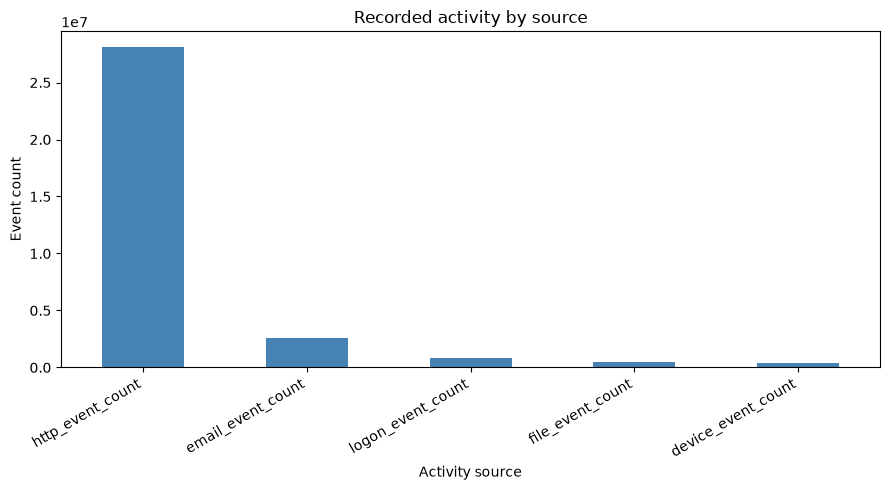
\includegraphics[width=0.79\textwidth,height=0.48\textheight,keepaspectratio]{notebook-1.png}
\caption{Retained activity events by source in the notebook analysis}
\label{fig:source-counts}
\end{figure}

\begin{figure}[H]
\centering
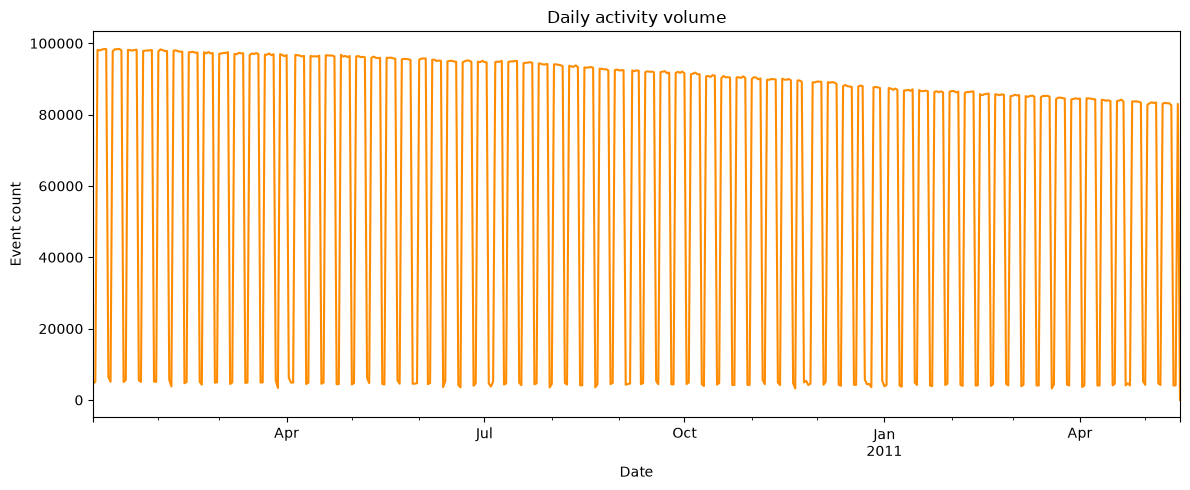
\includegraphics[width=0.9\textwidth,height=0.5\textheight,keepaspectratio]{notebook-2.png}
\caption{Daily recorded activity volume across the dataset period}
\label{fig:daily-counts}
\end{figure}

\begin{figure}[H]
\centering
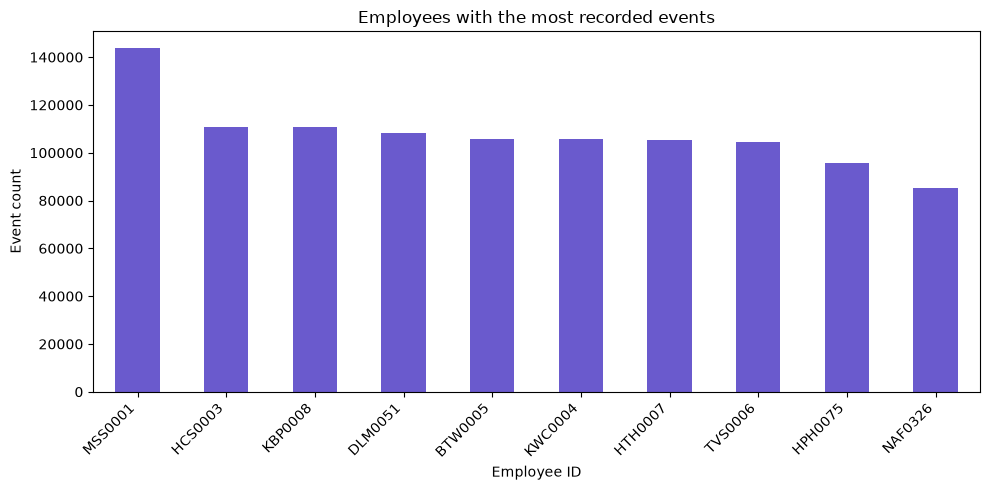
\includegraphics[width=0.83\textwidth,height=0.48\textheight,keepaspectratio]{notebook-3.png}
\caption{Ten synthetic users with the largest aggregate event counts}
\label{fig:top-users}
\end{figure}

\begin{figure}[H]
\centering
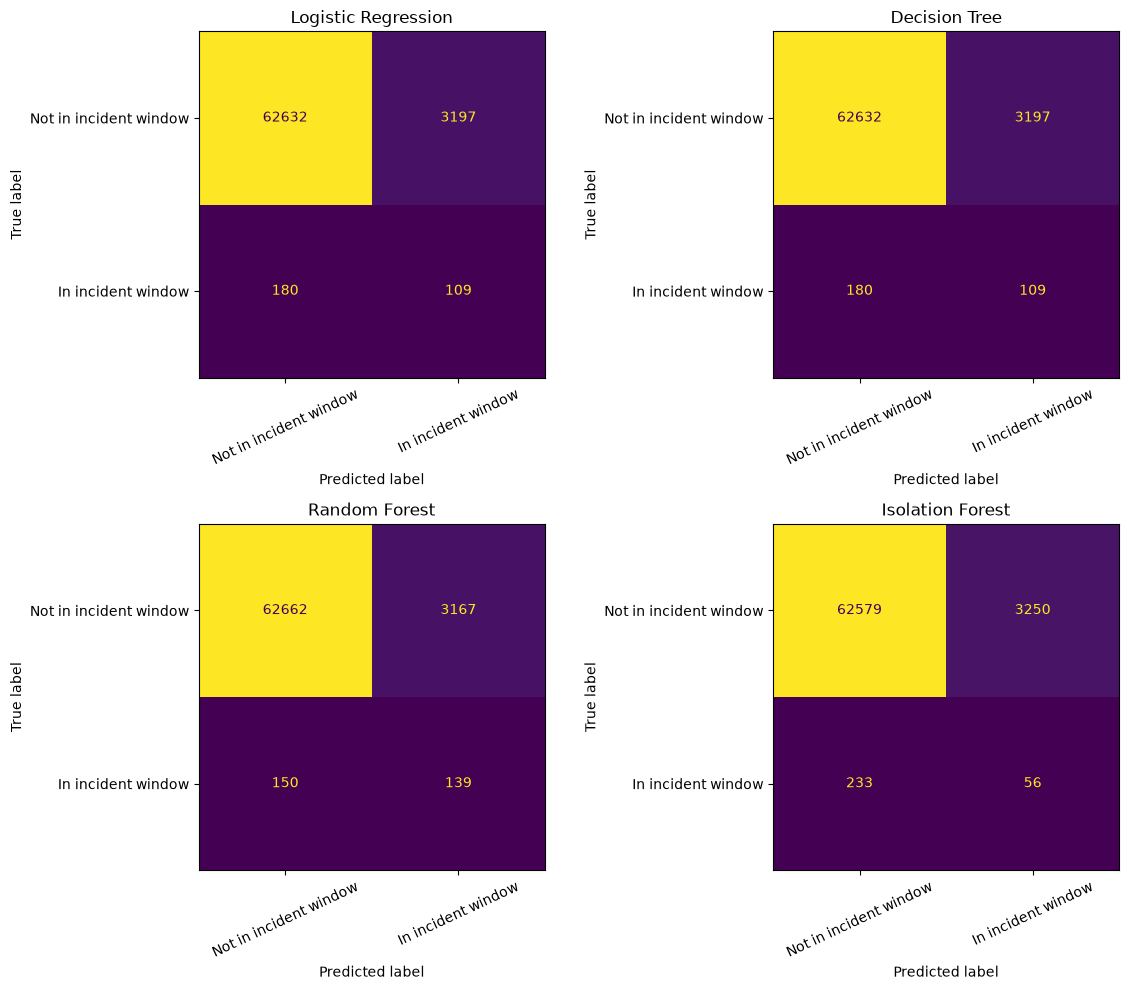
\includegraphics[width=0.85\textwidth,height=0.48\textheight,keepaspectratio]{notebook-4.png}
\caption{Model-evaluation visualization saved by the analysis notebook}
\label{fig:notebook-evaluation}
\end{figure}

The event-source plot shows why counts should be compared within an
appropriate feature and context. The daily series illustrates that
aggregate volume changes across the dataset period. The top-user chart
is not a list of suspicious employees. The evaluation visualization
must be read with the positive-class support and the review-capacity
rule; an attractive aggregate score cannot remove label uncertainty.

\section{Analysis of architecture and algorithms}

\subsection{Detailed study of the proposed algorithms}
\textbf{Logistic Regression.} The pipeline applies median imputation,
standard scaling, and a class-weighted Logistic Regression estimator.
The maximum iteration count is 1,000 and the random seed is fixed.
Scaling is important for a linear estimator when input counts have
different magnitudes. Class weighting gives the rare positive class
greater influence during fitting, but it does not by itself guarantee
high precision.

\textbf{Decision Tree.} The tree uses a maximum depth of 10, a minimum
leaf size of 10, balanced class weights, and a fixed random seed. Each
path through the tree applies feature thresholds. This can be easier to
explain than a large ensemble, but the model can still learn patterns
specific to its training data and does not provide causal explanations.

\textbf{Random Forest.} The forest contains 200 decision trees, uses a
minimum leaf size of 5, and applies
\code{balanced\_subsample} class weighting. Bootstrap variation and
aggregation can reduce the variance of an individual tree. In the
notebook, a real-data baseline is compared with an augmented candidate.
The augmented candidate is selected only when it improves validation
Average Precision. The saved comparison indicates 815 synthetic rows
were added to the selected Random Forest.

\textbf{Isolation Forest.} This model uses 200 estimators and automatic
contamination handling. It is fitted without incident labels and
assigns a lower decision function to more anomalous observations; the
pipeline reverses the sign so that larger values indicate greater
unusualness. Anomaly is not synonymous with harmful conduct, and this
model's score is not a probability.

\begin{table}[H]
\centering
\tablefont
\caption{Estimator configuration represented in the notebook}
\label{tab:model-settings}
\begin{tabularx}{\textwidth}{|p{0.23\textwidth}|p{0.33\textwidth}|Y|}
\hline
\textbf{Model} & \textbf{Configuration} & \textbf{Output used}\\\hline
Logistic Regression & Median imputation; standard scaling; class-weighted; 1,000 maximum iterations; seed 42. & Positive-class prediction score.\\\hline
Decision Tree & Maximum depth 10; minimum leaf size 10; balanced weights; seed 42. & Positive-class prediction score.\\\hline
Random Forest & 200 trees; minimum leaf size 5; balanced-subsample weights; parallel fitting; seed 42. & Positive-class prediction score; validation-selected baseline or augmented variant.\\\hline
Isolation Forest & 200 trees; automatic contamination; parallel fitting; seed 42. & Negative decision-function value, oriented so larger is more unusual.\\\hline
\end{tabularx}
\end{table}

\subsection{Step-by-step explanation of model operation}
The data flow begins with a feature matrix \(X\), binary incident-window
labels \(y\), and a user-group vector \(g\). A stratified group split
creates training, validation, and test partitions without sharing user
identifiers between them. Supervised models fit on training features
and labels. Isolation Forest fits only on training features.

For each candidate, a risk score is computed for validation data.
Random Forest compares a real-data fit to an augmented fit, where
positive training rows are resampled and count-perturbed. Validation
Average Precision selects between these variants. The notebook then
chooses a review capacity by searching candidate rates using validation
F1. Only after selection are test metrics calculated. The test set is
not used to choose the estimator or the queue rate.

\begin{enumerate}
  \item Construct and validate the employee-day feature matrix.
  \item Split groups of employees into training, validation, and test
  partitions using the notebook's stratified group splitters.
  \item Fit the four model families on training data, with labels
  supplied only to supervised models.
  \item Compare the Random Forest's baseline and augmented variants
  using validation Average Precision.
  \item Convert each score into a fixed-capacity decision for
  validation experiments and select the queue rate by validation F1.
  \item Evaluate selected estimators and operating capacity on
  untouched test data; retain both ranking metrics and confusion
  counts.
  \item Persist estimator objects, selected feature columns, and
  metadata in the model bundle for dashboard scoring.
\end{enumerate}

\subsection{Algorithm flow diagrams}
\begin{figure}[H]
\centering
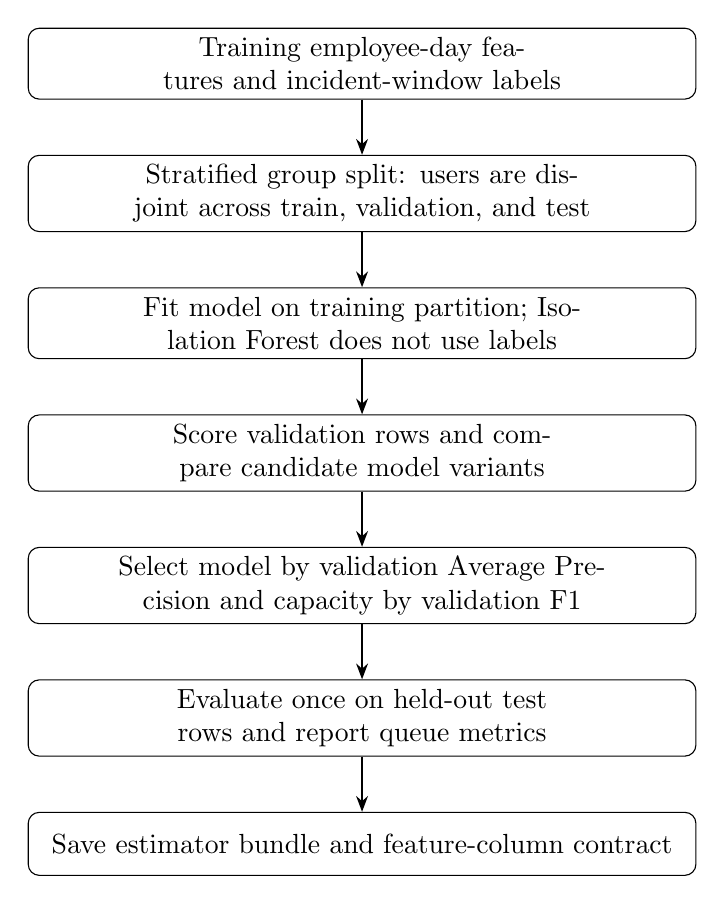
\begin{tikzpicture}[
  node distance=7mm and 10mm,
  box/.style={draw,rounded corners,align=center,text width=0.68\textwidth,minimum height=8mm},
  arrow/.style={-{Stealth[length=2mm]},thick}
]
\node[box] (data) {Training employee-day features and incident-window labels};
\node[box,below=of data] (split) {Stratified group split: users are disjoint across train, validation, and test};
\node[box,below=of split] (train) {Fit model on training partition; Isolation Forest does not use labels};
\node[box,below=of train] (valid) {Score validation rows and compare candidate model variants};
\node[box,below=of valid] (select) {Select model by validation Average Precision and capacity by validation F1};
\node[box,below=of select] (test) {Evaluate once on held-out test rows and report queue metrics};
\node[box,below=of test] (save) {Save estimator bundle and feature-column contract};
\draw[arrow] (data)--(split);
\draw[arrow] (split)--(train);
\draw[arrow] (train)--(valid);
\draw[arrow] (valid)--(select);
\draw[arrow] (select)--(test);
\draw[arrow] (test)--(save);
\end{tikzpicture}
\caption{Supervised training and evaluation flow}
\label{fig:training-flow}
\end{figure}

\begin{figure}[H]
\centering
\resizebox{\textwidth}{!}{%
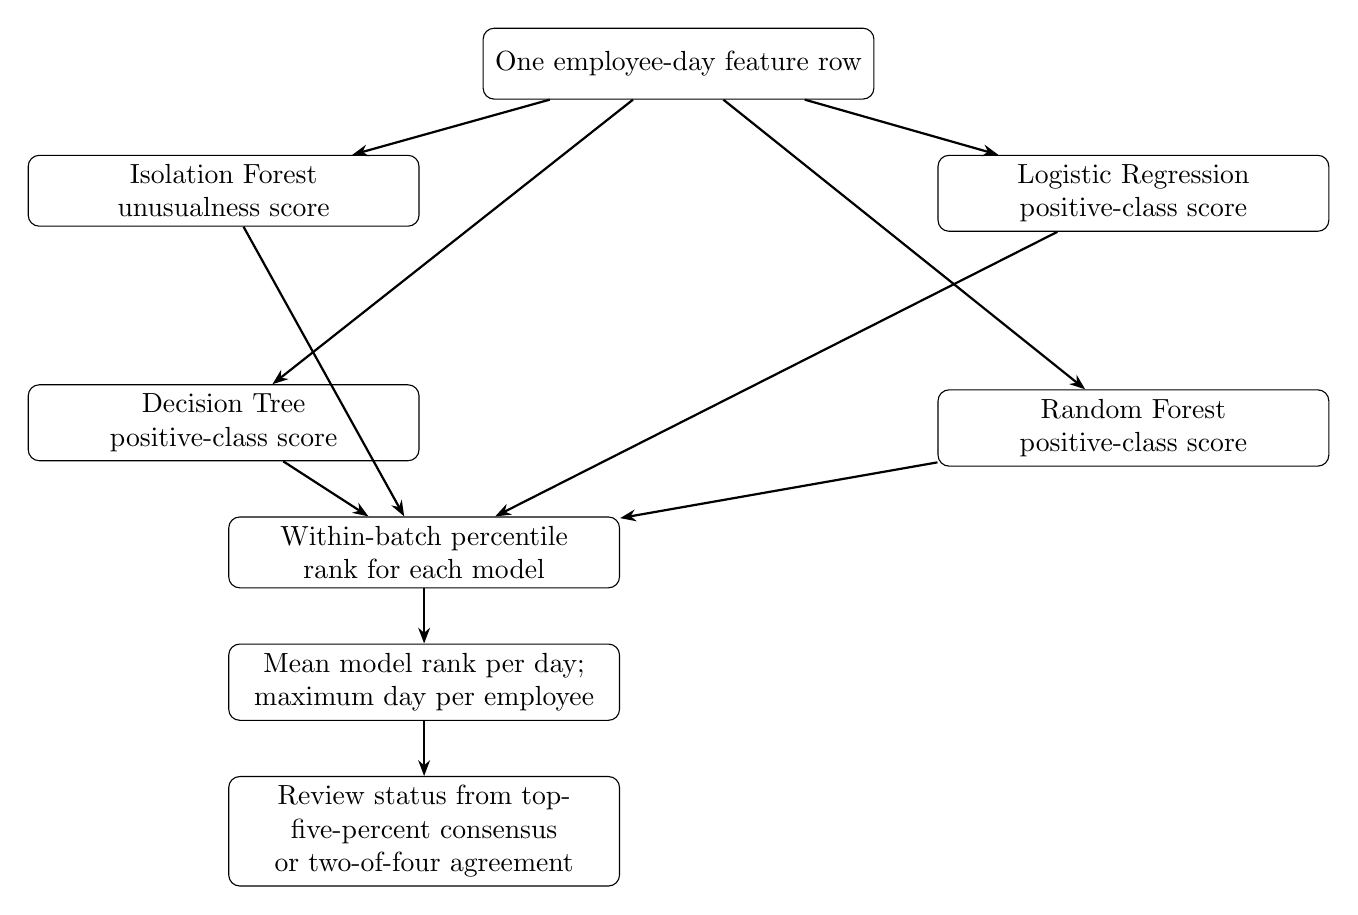
\begin{tikzpicture}[
  node distance=7mm and 8mm,
  box/.style={draw,rounded corners,align=center,text width=0.39\textwidth,minimum height=9mm},
  arrow/.style={-{Stealth[length=2mm]},thick}
]
\node[box] (input) {One employee-day feature row};
\node[box,below left=of input] (if) {Isolation Forest\\unusualness score};
\node[box,below right=of input] (lr) {Logistic Regression\\positive-class score};
\node[box,below=20mm of if] (dt) {Decision Tree\\positive-class score};
\node[box,below=20mm of lr] (rf) {Random Forest\\positive-class score};
\node[box,below=of dt,xshift=0.21\textwidth] (rank) {Within-batch percentile rank for each model};
\node[box,below=of rank] (mean) {Mean model rank per day; maximum day per employee};
\node[box,below=of mean] (queue) {Review status from top-five-percent consensus or two-of-four agreement};
\draw[arrow] (input)--(if);
\draw[arrow] (input)--(lr);
\draw[arrow] (input)--(dt);
\draw[arrow] (input)--(rf);
\draw[arrow] (if)--(rank);
\draw[arrow] (lr)--(rank);
\draw[arrow] (dt)--(rank);
\draw[arrow] (rf)--(rank);
\draw[arrow] (rank)--(mean);
\draw[arrow] (mean)--(queue);
\end{tikzpicture}%
}
\caption{Dashboard scoring and employee-level prioritisation}
\label{fig:ensemble-flow}
\end{figure}

The dashboard first creates percentile ranks separately within the
current scoring batch because the model outputs are on different
scales. A per-day consensus is the mean of the four ranks. The employee
table uses the highest daily consensus for each user and each model's
highest employee-level rank. The display status is set when consensus
is within the top five percent of employees or at least two model
ranks are in their respective top ten percent. This rule is intended
to prioritise review, not to classify guilt.

\section{Project pipeline}
\begin{figure}[H]
\centering
\resizebox{\textwidth}{!}{%
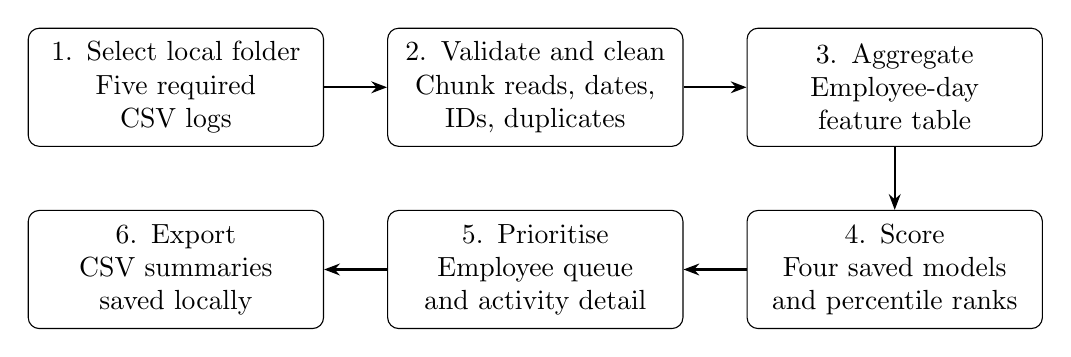
\begin{tikzpicture}[
  node distance=8mm and 8mm,
  stage/.style={draw,rounded corners,align=center,text width=0.29\textwidth,minimum height=15mm},
  arrow/.style={-{Stealth[length=2mm]},thick}
]
\node[stage] (input) {1. Select local folder\\Five required CSV logs};
\node[stage,right=of input] (clean) {2. Validate and clean\\Chunk reads, dates, IDs, duplicates};
\node[stage,right=of clean] (aggregate) {3. Aggregate\\Employee-day feature table};
\node[stage,below=of aggregate] (score) {4. Score\\Four saved models and percentile ranks};
\node[stage,left=of score] (review) {5. Prioritise\\Employee queue and activity detail};
\node[stage,left=of review] (export) {6. Export\\CSV summaries saved locally};
\draw[arrow] (input)--(clean);
\draw[arrow] (clean)--(aggregate);
\draw[arrow] (aggregate)--(score);
\draw[arrow] (score)--(review);
\draw[arrow] (review)--(export);
\end{tikzpicture}%
}
\caption{End-to-end project pipeline}
\label{fig:project-pipeline}
\end{figure}

\subsection{Explanation of pipeline stages}
\textbf{Input selection.} The React client gathers files from a selected
folder and posts the expected CSVs to the local API. An alternative
API endpoint accepts a folder path on the host. The application expects
the five source filenames exactly, apart from case normalisation in
upload handling.

\textbf{Validation and cleaning.} Required source presence is checked
before scoring. Each log is streamed in chunks and normalised to the
columns the aggregator needs. Missing required columns or unreadable
records cause explicit errors rather than a successful-looking empty
report.

\textbf{Aggregation and alignment.} Each source becomes a user-day
table. Tables are aligned on user and day, missing source-day
contributions are filled with zero, and the final feature matrix is
reordered to the saved feature list. This ordering is critical because
estimators bind learned parameters to column positions.

\textbf{Scoring and ranking.} Every estimator processes the same
feature matrix. Scores are converted to percentile ranks, averaged per
employee-day, and reduced to employee-level maxima. The system builds
human-readable reasons from selected high-volume signals on the
highest-consensus day.

\textbf{Review and export.} The dashboard provides a ranked queue,
summary metrics, filtering, search, per-model scores, and a short
activity table. The API and Streamlit app write day-level and
employee-level CSV outputs into \code{sprint1\_output}. The outputs are
local demonstration artifacts and are not an immutable evidence store.

\section{Feasibility analysis}

\subsection{Technical feasibility}
The system is technically feasible as a local prototype because its
components use widely available Python and JavaScript tooling, its
inputs are ordinary CSV files, and model training can be performed
offline. The scorer limits individual CSV reads to 25,000-row chunks.
The overall workflow still holds grouped and scored data in memory, so
the project has not demonstrated arbitrary-scale streaming. Runtime
and memory should be benchmarked on the target machine and data volume.

\subsection{Economic feasibility}
The software stack relies on open-source packages and a local
development environment. No hosted service, paid API, or dedicated
database is required for the demonstration. Costs remain in personnel
time, workstation resources, data governance, security review,
maintenance, and any organisational licensing or infrastructure
requirements. Open-source availability does not eliminate the cost of
operating a responsible investigation process.

\subsection{Operational feasibility}
An analyst can select a folder, run analysis, inspect a queue, and
review activity aggregates without learning the model code. The
prototype provides an understandable entry point, but it does not
support case assignment, audit trails, reviewer notes, approvals, or
incident-system integration. Operational deployment would require
those controls and a written process for challenging, documenting, and
closing a review.

\begin{table}[H]
\centering
\tablefont
\caption{Feasibility summary}
\label{tab:feasibility}
\begin{tabularx}{\textwidth}{|p{0.20\textwidth}|Y|Y|}
\hline
\textbf{Dimension} & \textbf{Current position} & \textbf{Condition for broader use}\\\hline
Technical & Local Python/API/browser stack and serialized models work as a coherent prototype. & Benchmark full data volume; add schema validation, failure recovery, and monitoring.\\\hline
Economic & No external paid service is required for the demonstration. & Budget for review staff, secure endpoints, maintenance, and governance.\\\hline
Operational & Folder selection and ranked review are straightforward. & Add case workflow, auditability, accountable reviewers, and escalation policy.\\\hline
Privacy & Feature generation omits content fields and processing is local by design. & Enforce access, retention, consent/legal basis, and secure handling of source logs.\\\hline
\end{tabularx}
\end{table}

\section{System environment}

\subsection{Software environment}
The Python backend depends on pandas, NumPy, scikit-learn, joblib,
FastAPI, Pydantic through FastAPI, python-multipart, and Uvicorn.
Streamlit is used by the alternative interface. The browser client
uses React and Vite. Exact dependency versions should be captured in a
lock file for a reproducible deployment; the repository's current
requirements file lists package names without strict versions.

\subsection{Hardware environment}
The demonstrated setup is a developer workstation capable of running
Python, a local web service, and a browser. The saved model bundle and
large data files determine the actual memory and storage requirements.
No measured minimum CPU, RAM, disk, or runtime benchmark is included in
the repository; the hardware values in Appendix 10.1 are therefore
presented as practical setup guidance, not measured guarantees.

\section{Actors and roles}
\begin{table}[H]
\centering
\tablefont
\caption{Actors and responsibilities}
\label{tab:actors}
\begin{tabularx}{\textwidth}{|p{0.22\textwidth}|p{0.36\textwidth}|Y|}
\hline
\textbf{Actor} & \textbf{Responsibilities} & \textbf{System boundary}\\\hline
Analyst / operator & Select a dataset, run analysis, inspect ranked signals, verify source evidence, document a review. & The prototype supports selection and inspection; investigation decisions remain external.\\\hline
Data custodian & Authorise use of input logs and ensure correct scope and retention. & Not implemented as an application role; required operational control.\\\hline
Model maintainer & Build and version the model bundle, record evaluation and feature schema, assess changes. & Notebook and model artifacts support development; no registry is present.\\\hline
Application operator & Start the local API and browser client, monitor errors, protect outputs. & Local developer workflow; production service controls are out of scope.\\\hline
\end{tabularx}
\end{table}

\section{Functional and non-functional requirements}
\begin{longtable}{|p{0.12\textwidth}|p{0.39\textwidth}|p{0.14\textwidth}|p{0.24\textwidth}|}
\caption{Functional and non-functional requirements}\label{tab:requirements}\\
\hline
\textbf{ID} & \textbf{Requirement} & \textbf{Class} & \textbf{Evidence in project}\\\hline
\endfirsthead
\hline
\textbf{ID} & \textbf{Requirement} & \textbf{Class} & \textbf{Evidence in project}\\\hline
\endhead
\hline
\multicolumn{4}{r}{Continued on next page}\\
\endfoot
\hline
\endlastfoot
FR-01 & Accept the five required activity sources and report missing files. & Functional & API upload validation and scorer file checks.\\\hline
FR-02 & Process records with bounded chunk reads. & Functional & Core CSV processor uses 25,000-row chunks.\\\hline
FR-03 & Reproduce the trained employee-day feature schema. & Functional & Model bundle stores \code{feature\_columns}.\\\hline
FR-04 & Score each employee-day with four estimator families. & Functional & Core scoring loop iterates through model names.\\\hline
FR-05 & Present employee-level priorities and a reason summary. & Functional & API response and dashboard queue.\\\hline
FR-06 & Show activity detail for a selected employee. & Functional & Employee endpoint returns up to 20 ranked days.\\\hline
FR-07 & Export day-level and employee-level CSV summaries. & Functional & Output files are written to \code{sprint1\_output}.\\\hline
NFR-01 & Keep the demonstration local by default. & Non-functional & API binds to loopback in the documented run configuration.\\\hline
NFR-02 & Distinguish relative ranks from probabilities or proof. & Non-functional & Dashboard text and report disclaimers.\\\hline
NFR-03 & Fail visibly when data or model prerequisites are missing. & Non-functional & API returns errors and UI displays failures.\\\hline
NFR-04 & Preserve understandable source-to-feature lineage. & Non-functional & Source-specific aggregate definitions are documented.\\\hline
NFR-05 & Support reproducible evaluation. & Non-functional & Fixed random seeds and saved evaluation artifacts.\\\hline
NFR-06 & Protect sensitive data at rest and in transit. & Non-functional & Not fully implemented; a deployment prerequisite.\\\hline
\end{longtable}

\chapter{System design}
\label{chap:design}

\section{Model building}
Model development and model deployment are separate stages. The
notebook uses labelled synthetic activity for training and
evaluation. The deployed local scorer accepts unlabeled activity,
loads an already-created bundle, and produces a ranked report. The
dashboard does not retrain estimators when an analyst submits a folder.

\subsection{Implementation code}
Notebook cells implement data inspection, aggregation, label
construction, group splitting, model fitting, validation selection,
test evaluation, visualisation, and bundle persistence. The scoring
core shares the feature-generation contract used by the application.
The selected feature list is included in the bundle so the inference
path can insert missing columns and order inputs consistently.

\subsection{Model planning and training/testing split}
The notebook applies an outer \code{StratifiedGroupKFold} splitter with
five folds and a fixed seed to hold out test users. An inner
four-fold stratified group split with a separate seed partitions the
remaining users into training and validation groups. The first
split produced by each configured splitter is used. The identifier
groups are checked for overlap. If any partition lacks a positive
employee-day, the notebook stops rather than reporting an unusable
comparison.

The saved evaluation partition contains 66,118 employee-days and 289
positive rows. The group split is a stronger safeguard against
same-user leakage than a random row split, though it does not solve
temporal drift, release-to-release shift, or differences between
synthetic and real activity.

\subsection{Training}
The supervised estimators are fitted on training labels only.
Isolation Forest is fitted on training features and does not use the
incident labels. The Random Forest augmentation routine creates one
count-perturbed positive example per positive training row. It samples
positive anchors, applies a log-normal multiplier, resamples event
counts from Poisson distributions, and reconstructs after-hours,
device-connection, and attachment counts while preserving
source-level relationships. Validation Average Precision decides
whether the augmented version is retained. Test data is not used for
that decision.

\subsection{Testing}
The notebook evaluates the selected estimators on the held-out test
partition. It chooses the queue rate on validation data by searching a
set of candidate capacities and maximising validation F1. The saved
rate is one percent. At that rate the test set contributes 662
employee-days to the queue. A five-percent capacity is also retained
as a comparison reference. These are ranking capacities, not fixed
probability thresholds.

\section{System architecture}
\begin{figure}[H]
\centering
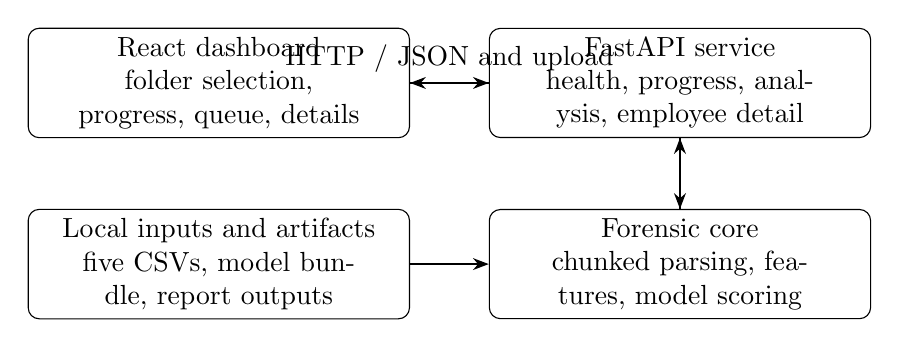
\begin{tikzpicture}[
  node distance=9mm and 10mm,
  unit/.style={draw,rounded corners,align=center,text width=0.38\textwidth,minimum height=12mm},
  arrow/.style={-{Stealth[length=2mm]},thick}
]
\node[unit] (browser) {React dashboard\\folder selection, progress, queue, details};
\node[unit,right=of browser] (api) {FastAPI service\\health, progress, analysis, employee detail};
\node[unit,below=of api] (core) {Forensic core\\chunked parsing, features, model scoring};
\node[unit,left=of core] (files) {Local inputs and artifacts\\five CSVs, model bundle, report outputs};
\draw[arrow] (browser)--node[above]{HTTP / JSON and upload}(api);
\draw[arrow] (api)--(core);
\draw[arrow] (files)--(core);
\draw[arrow] (core)--(api);
\draw[arrow] (api)--(browser);
\end{tikzpicture}
\caption{Application component architecture}
\label{fig:architecture}
\end{figure}

\subsection{Component responsibilities}
\textbf{React client.} The client checks health, collects files using a
directory input, uploads the selected CSVs, polls progress, and
renders the report. It supports employee search and status filtering,
and requests activity detail for a selected employee.

\textbf{FastAPI service.} The service validates uploaded filenames,
stages accepted files in a temporary directory, invokes the scoring
core, stores the most recent in-memory results for detail requests,
and writes CSV exports. It exposes health and progress endpoints for
the UI. A lock serialises analysis requests in this single-process
prototype.

\textbf{Forensic core.} The core checks model availability and required
input files, parses the logs in chunks, builds user-day features,
orders model inputs, scores with each estimator, calculates consensus
ranks, generates reasons, and formats selected activity rows.

\textbf{Model bundle.} The bundle contains the four fitted models and
the feature-column list. It is loaded with joblib. Bundle files are
trusted local artifacts; loading joblib from an untrusted source is
not safe and must not be permitted in an operational deployment.

\section{Use-case model}
\begin{figure}[H]
\centering
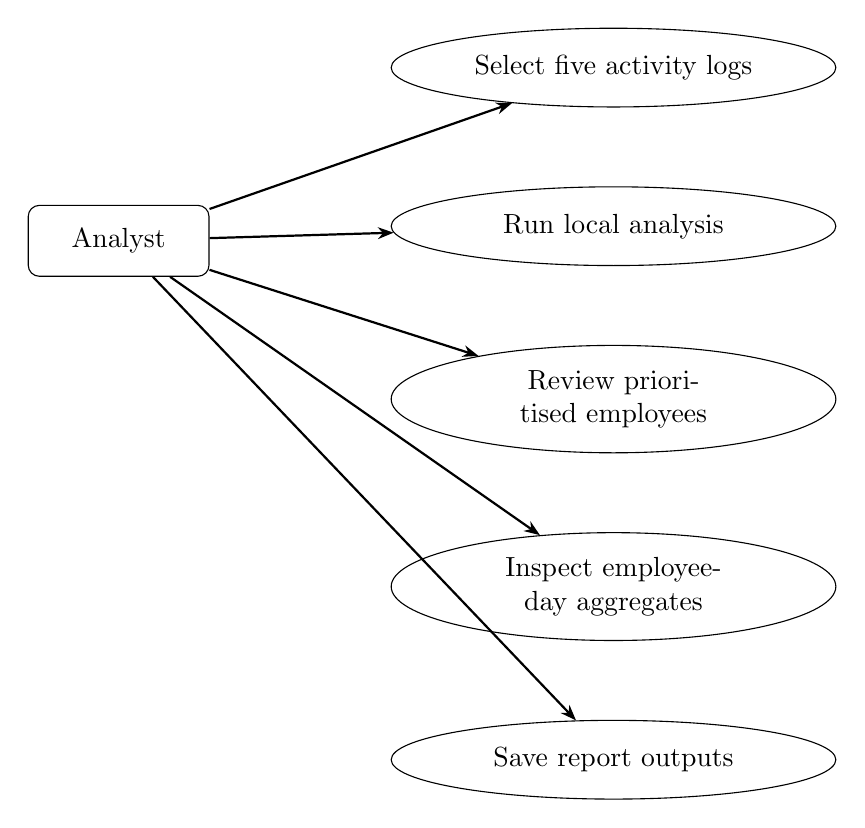
\begin{tikzpicture}[
  usecase/.style={draw,ellipse,align=center,text width=0.31\textwidth,minimum height=10mm},
  actor/.style={draw,rounded corners,align=center,text width=0.17\textwidth,minimum height=9mm},
  arrow/.style={-{Stealth[length=2mm]},thick}
]
\node[actor] (analyst) {Analyst};
\node[usecase,right=23mm of analyst,yshift=22mm] (select) {Select five activity logs};
\node[usecase,below=of select] (run) {Run local analysis};
\node[usecase,below=of run] (queue) {Review prioritised employees};
\node[usecase,below=of queue] (detail) {Inspect employee-day aggregates};
\node[usecase,below=of detail] (export) {Save report outputs};
\draw[arrow] (analyst)--(select);
\draw[arrow] (analyst)--(run);
\draw[arrow] (analyst)--(queue);
\draw[arrow] (analyst)--(detail);
\draw[arrow] (analyst)--(export);
\end{tikzpicture}
\caption{Primary analyst use cases}
\label{fig:use-case}
\end{figure}

The analyst is the principal interactive actor. Data custodians and
model maintainers are operational stakeholders but are not
authenticated application roles. The use-case diagram intentionally
does not model automated decision-making: the application ranks
records and exposes information for a human process outside the
prototype.

\section{Activity diagram}
\begin{figure}[H]
\centering
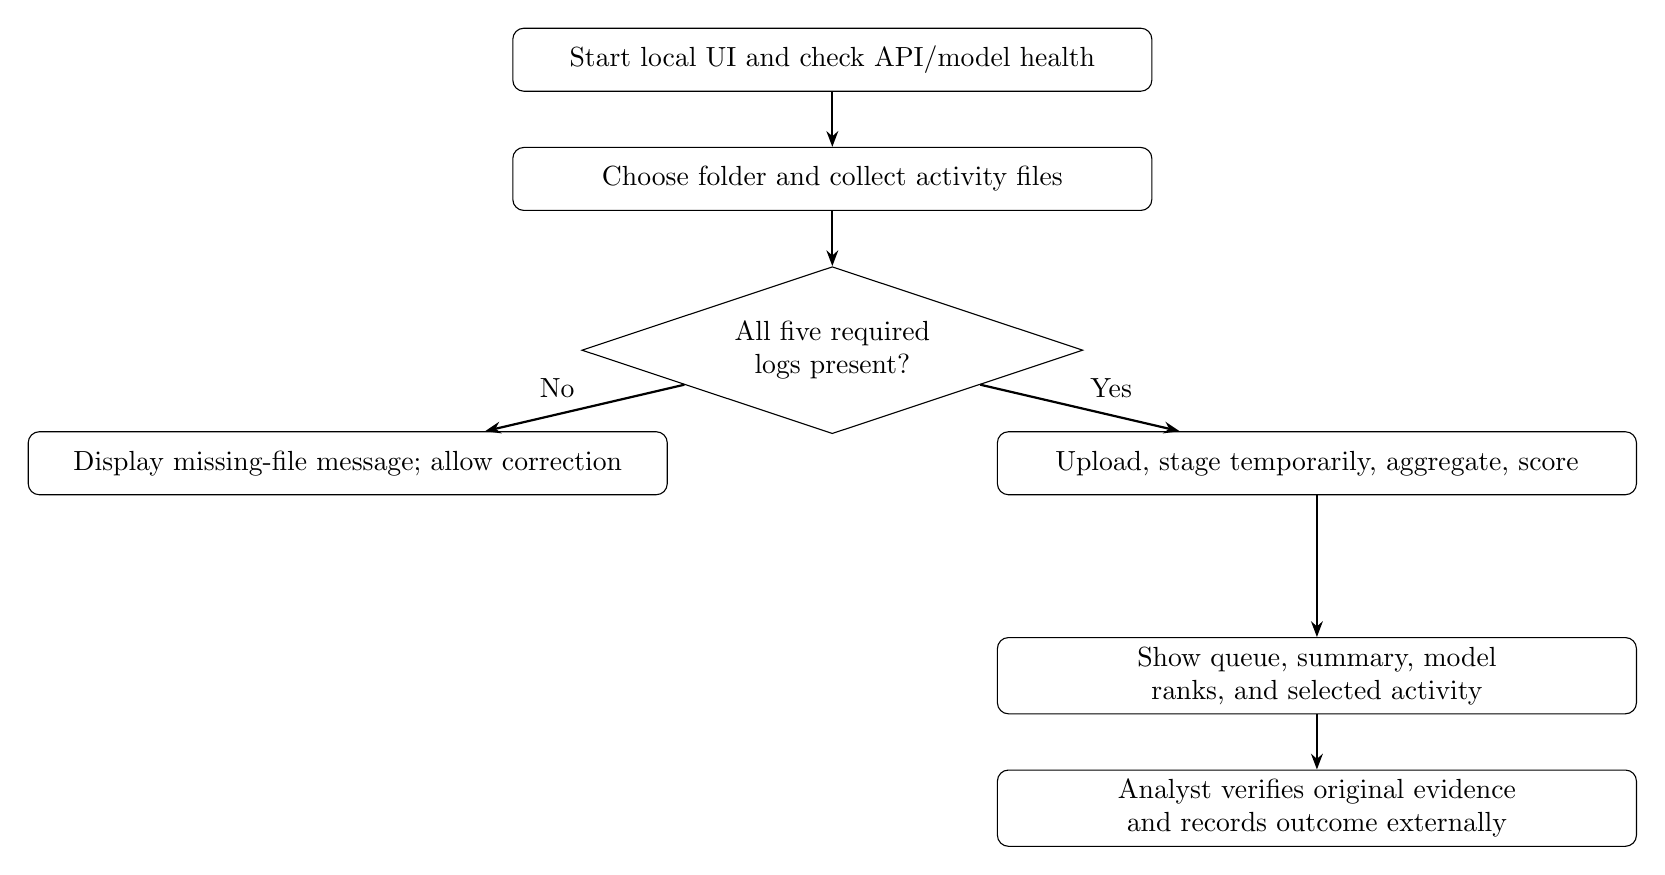
\begin{tikzpicture}[
  node distance=7mm,
  process/.style={draw,rounded corners,align=center,text width=0.65\textwidth,minimum height=8mm},
  decision/.style={draw,diamond,aspect=3,align=center,text width=0.32\textwidth,inner sep=1pt},
  arrow/.style={-{Stealth[length=2mm]},thick}
]
\node[process] (start) {Start local UI and check API/model health};
\node[process,below=of start] (choose) {Choose folder and collect activity files};
\node[decision,below=of choose] (complete) {All five required logs present?};
\node[process,below left=of complete] (error) {Display missing-file message; allow correction};
\node[process,below right=of complete] (upload) {Upload, stage temporarily, aggregate, score};
\node[process,below=18mm of upload] (show) {Show queue, summary, model ranks, and selected activity};
\node[process,below=of show] (end) {Analyst verifies original evidence and records outcome externally};
\draw[arrow] (start)--(choose);
\draw[arrow] (choose)--(complete);
\draw[arrow] (complete)--node[above left]{No}(error);
\draw[arrow] (complete)--node[above right]{Yes}(upload);
\draw[arrow] (upload)--(show);
\draw[arrow] (show)--(end);
\end{tikzpicture}
\caption{Analysis and review activity}
\label{fig:activity}
\end{figure}

\section{Sequence diagram}
\begin{figure}[H]
\centering
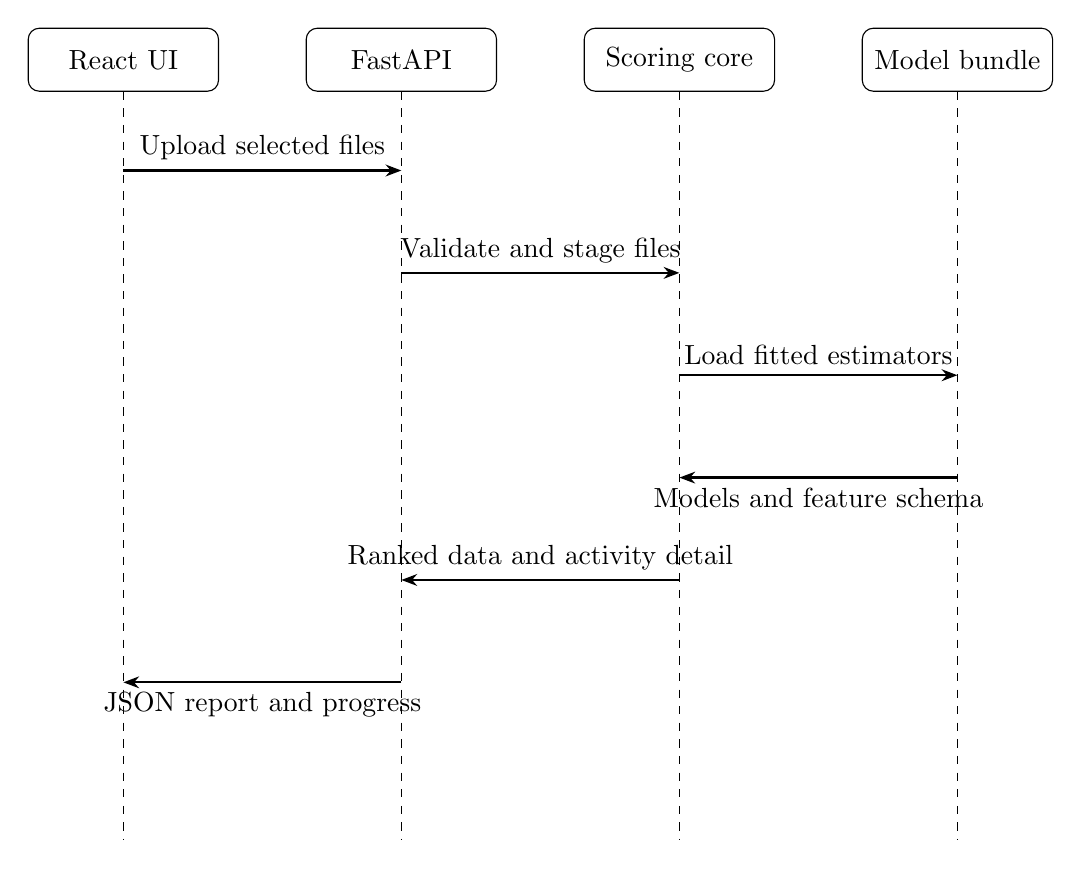
\begin{tikzpicture}[
  actor/.style={draw,rounded corners,align=center,text width=0.18\textwidth,minimum height=8mm},
  arrow/.style={-{Stealth[length=2mm]},thick},
  node distance=10mm and 11mm
]
\node[actor] (ui) {React UI};
\node[actor,right=of ui] (api) {FastAPI};
\node[actor,right=of api] (core) {Scoring core};
\node[actor,right=of core] (bundle) {Model bundle};
\draw[dashed] (ui.south)--++(0,-9.5);
\draw[dashed] (api.south)--++(0,-9.5);
\draw[dashed] (core.south)--++(0,-9.5);
\draw[dashed] (bundle.south)--++(0,-9.5);
\draw[arrow] ([yshift=-10mm]ui.south)--node[above]{Upload selected files}([yshift=-10mm]api.south);
\draw[arrow] ([yshift=-23mm]api.south)--node[above]{Validate and stage files}([yshift=-23mm]core.south);
\draw[arrow] ([yshift=-36mm]core.south)--node[above]{Load fitted estimators}([yshift=-36mm]bundle.south);
\draw[arrow] ([yshift=-49mm]bundle.south)--node[below]{Models and feature schema}([yshift=-49mm]core.south);
\draw[arrow] ([yshift=-62mm]core.south)--node[above]{Ranked data and activity detail}([yshift=-62mm]api.south);
\draw[arrow] ([yshift=-75mm]api.south)--node[below]{JSON report and progress}([yshift=-75mm]ui.south);
\end{tikzpicture}
\caption{High-level sequence for a folder analysis}
\label{fig:sequence}
\end{figure}

\section{Data design}
The project uses file-based input and output rather than a relational
database. The main logical records are source events, employee-day
aggregates, model scores, employee summaries, and optional display
names. A user-day key joins the source aggregates. The user key joins
day rows to an employee summary.

\begin{table}[H]
\centering
\tablefont
\caption{Logical data entities}
\label{tab:entities}
\begin{tabularx}{\textwidth}{|p{0.23\textwidth}|p{0.30\textwidth}|Y|}
\hline
\textbf{Entity} & \textbf{Key fields} & \textbf{Purpose}\\\hline
Source event & user, timestamp, source-specific fields & Original observed event; retained in input files.\\\hline
Employee-day row & user, day, feature columns & Aggregated evidence used by the estimators.\\\hline
Model score row & user, day, four model ranks, consensus & Relative model ranking for one employee-day.\\\hline
Employee summary & user, active days, maxima, agreement, status & Review queue record and explanatory summary.\\\hline
Name lookup & user, name & Optional display-only lookup; not used as model input.\\\hline
\end{tabularx}
\end{table}

The service stores the last successful analysis in process memory for
employee-detail requests. The in-memory state is not durable, is
shared only within the running process, and is replaced by the next
analysis. The CSV exports are convenient report artifacts but do not
include a transactional case history. A production design should
define stable identifiers, access permissions, retention periods,
integrity checks, backup policy, and an append-only audit trail.

\section{API design}
\begin{table}[H]
\centering
\tablefont
\caption{Local API endpoints}
\label{tab:api}
\begin{tabularx}{\textwidth}{|p{0.19\textwidth}|p{0.28\textwidth}|p{0.42\textwidth}|}
\hline
\textbf{Method and route} & \textbf{Purpose} & \textbf{Result and error behaviour}\\\hline
\code{GET /api/health} & Report model-bundle readiness. & Returns a readiness Boolean and explanatory message.\\\hline
\code{GET /api/progress} & Read current analysis stage. & Returns percentage, stage text, and active state.\\\hline
\code{POST /api/analyze} & Analyse an existing local folder path. & Returns employee records and summary; invalid folders or scoring failures return errors.\\\hline
\code{POST /api/analyze-upload} & Receive selected activity files. & Validates required names, rejects duplicates, stages files temporarily, and returns ranked results.\\\hline
\code{POST /api/employee} & Request detail for one user. & Returns model scores and selected daily activity; returns conflict before analysis or not-found for unknown users.\\\hline
\end{tabularx}
\end{table}

The browser uses the upload route so the backend can operate on a
temporary staged folder. File names are reduced to their basename and
compared with an allowlist of required and optional names. This is a
useful input constraint, but it is not a complete security boundary:
the application has no user authentication, rate limiting, CSRF
protection, or production-grade isolation. It is documented to run on
the loopback interface and should not be exposed to an untrusted
network.

\section{UI design}
The React interface uses a dark sidebar, a light review workspace, a
folder-selection card, an expandable model guide, and an analysis
progress panel. After scoring, the dashboard presents summary counts,
flagged employees, a searchable directory, and employee activity
details. Status language is deliberately framed as review priority.

\begin{figure}[H]
\centering
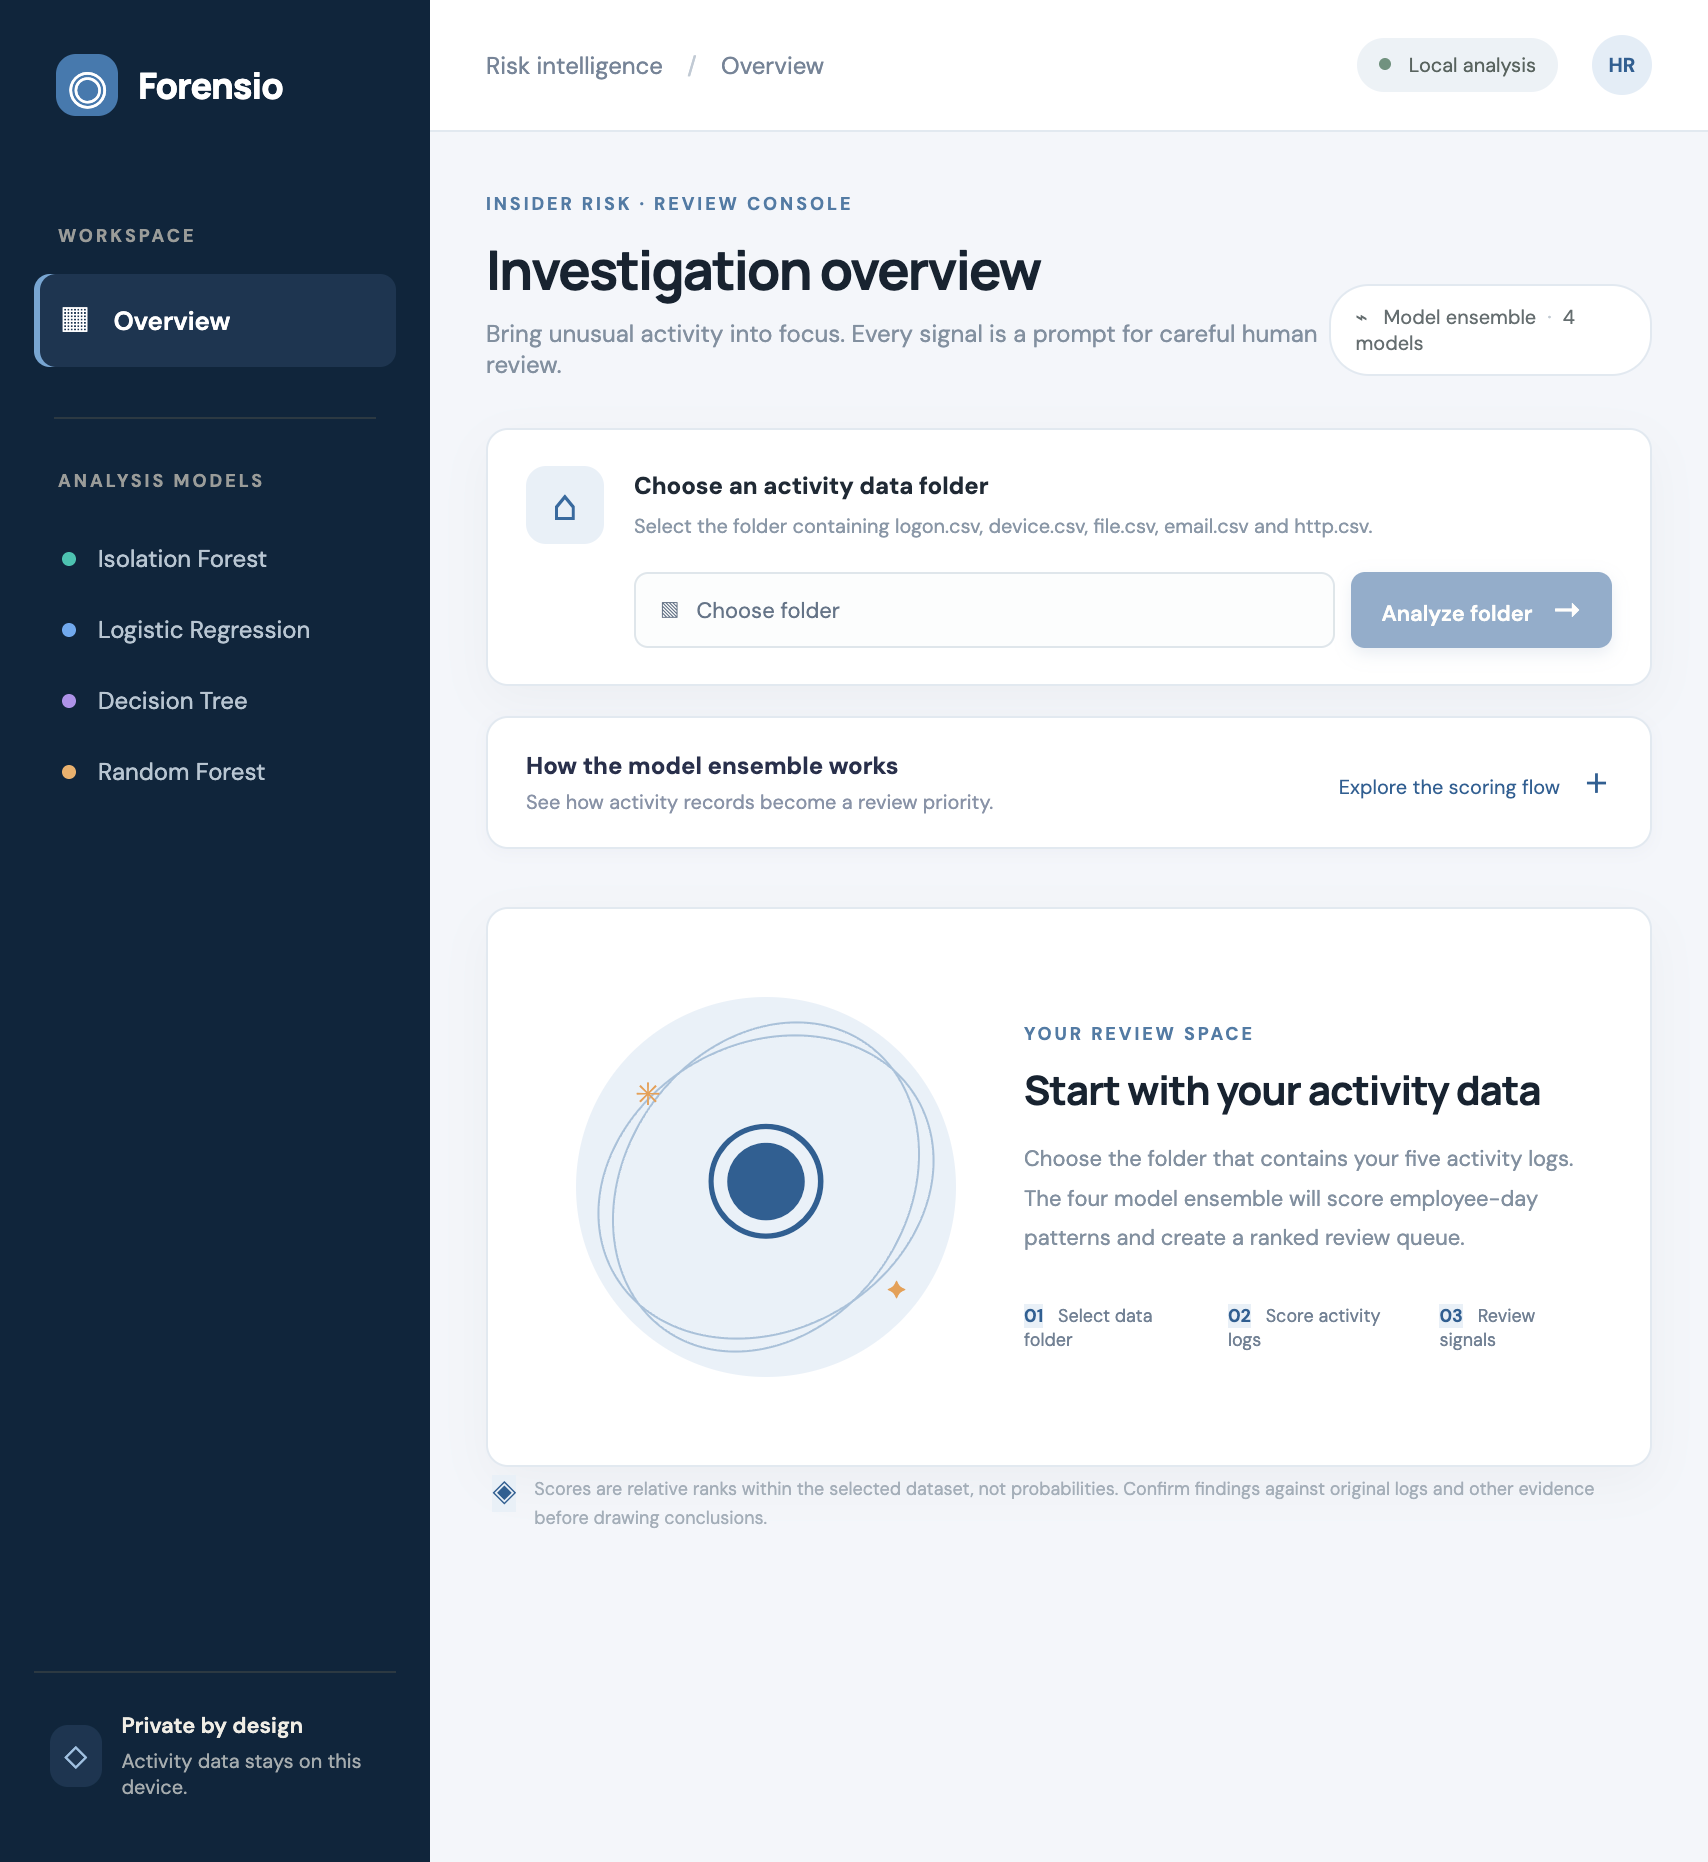
\includegraphics[width=0.78\textwidth,height=0.65\textheight,keepaspectratio]{ui_react_landing.png}
\caption{Forensio React dashboard landing state}
\label{fig:ui-landing}
\end{figure}

\begin{figure}[H]
\centering
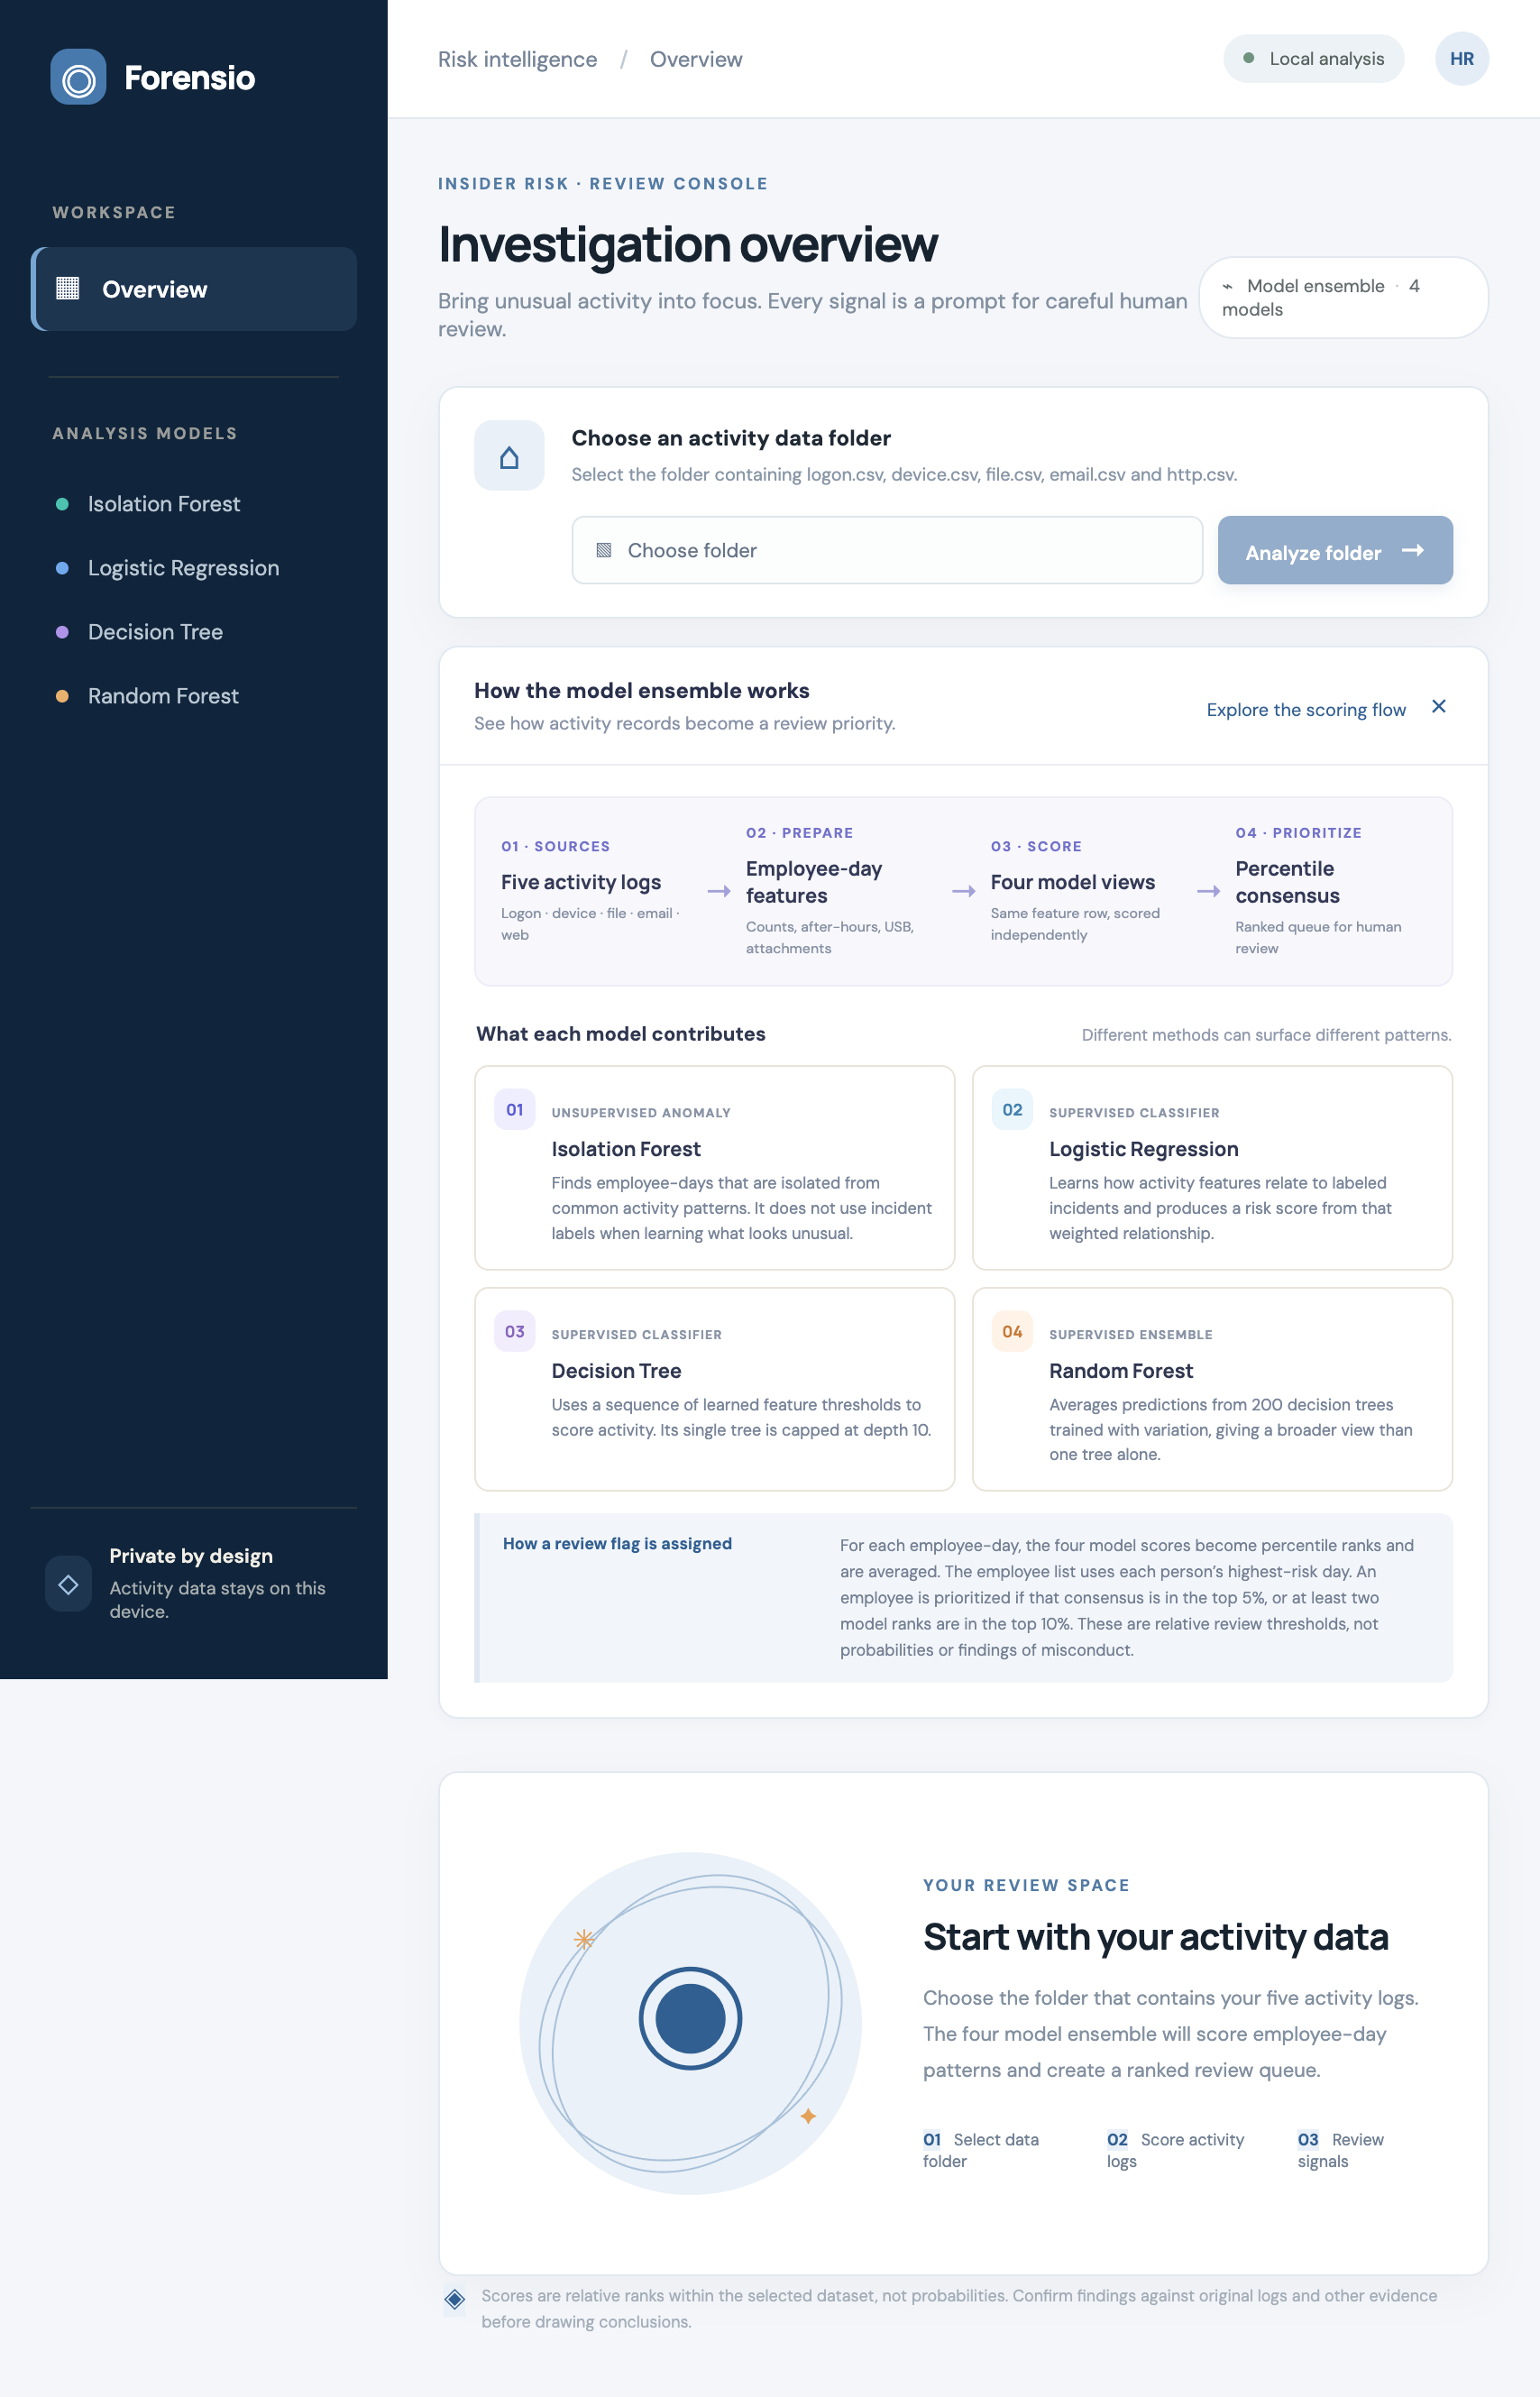
\includegraphics[width=0.69\textwidth,height=0.72\textheight,keepaspectratio]{ui_react_model_guide.png}
\caption{Expanded model guide and scoring explanation}
\label{fig:ui-guide}
\end{figure}

The landing screenshot illustrates the initial local-analysis state.
The model-guide screenshot describes the four methods and the
percentile-based dashboard rule. Captures are snapshots of the
interface and may not show every interaction state or the latest visual
change. The report does not treat a screenshot as proof that every
workflow has been tested end to end.

\subsection{Interaction states}
\begin{table}[H]
\centering
\tablefont
\caption{User-interface states and visible response}
\label{tab:ui-states}
\begin{tabularx}{\textwidth}{|p{0.21\textwidth}|p{0.37\textwidth}|Y|}
\hline
\textbf{State} & \textbf{Trigger} & \textbf{Expected interface response}\\\hline
Checking service & Page load or API not reachable. & Show availability message and retry the health request.\\\hline
Ready & Model bundle is present and API is reachable. & Enable folder selection and analysis when required inputs are found.\\\hline
Incomplete folder & One or more required CSVs are absent. & List the missing filenames and disable analysis.\\\hline
Uploading & Browser sends selected files. & Display upload progress and disable repeated submission.\\\hline
Scoring & API aggregates and scores records. & Poll progress and show current stage and estimated remaining time.\\\hline
Successful analysis & API returns a report. & Render summary, flagged queue, searchable directory, and details.\\\hline
Failed analysis & Service or parser returns an error. & Show an error message so the operator can correct input or inspect service logs.\\\hline
\end{tabularx}
\end{table}

\subsection{Accessibility and usability}
The React implementation uses native form controls, descriptive labels
for the directory picker, a live status region for analysis progress,
and a progress bar with current and maximum values. Search and status
filters reduce navigation effort when the employee list is large. A
textual model guide explains the distinction between model families
and the review rule.

Further accessibility work should include keyboard-only workflow
testing, focus management after analysis, screen-reader testing of
dynamic results, high-contrast verification, and clear focus
indicators. The current screenshots are visual evidence of layout,
not a formal accessibility conformance assessment.

\chapter{Results and discussion}
\label{chap:results}

\section{Testing approach}
The repository contains saved data-quality and evaluation artifacts,
but no dedicated automated test suite was identified. This report
therefore distinguishes checks reflected in the source and saved
outputs from tests that would still need to be run. The test cases in
Appendix 10.4 are a verification plan unless an execution result is
explicitly recorded. They must not be interpreted as all passing.

The strongest available quantitative evidence is the saved
employee-day model comparison and confusion-count output. The saved
training notebook fixes random seeds for splitting and estimators;
however, reproducibility also depends on package versions, data-file
integrity, notebook execution order, and model artifact provenance.

\section{Model planning and evaluation protocol}
The labelled table contains 330,452 employee-days and 1,364 positives.
The held-out test partition has 66,118 employee-days, including 289
positives. The selected queue size is 662 rows at one percent. The
one-percent capacity was selected on validation data only by F1 search;
the estimator variant was selected on validation Average Precision.
The test split was reserved for reporting.

Evaluation is made at the employee-day level. The test confusion
matrix describes whether a row is inside a known incident interval
under the answer-file label rule. It does not state whether a person
committed misconduct, nor does it establish the correctness of an
investigative outcome.

\section{Validation design and class imbalance}
The saved employee-day table is strongly imbalanced: 1,364 of 330,452
rows are positive under the incident-window rule. A model can therefore
rank a large number of ordinary-looking records above the rare positive
class without a large change in overall accuracy. This affects both
training and evaluation. Class weighting changes the penalty associated
with misclassified examples during supervised fitting, but it does not
create new independent incidents. Synthetic augmentation adds derived
training examples according to a transformation rule; it must not be
counted as additional observed evidence.

The project uses user-group separation so that records from one
synthetic person are not split across training, validation, and test.
This addresses a specific leakage risk: daily rows from one user may
share activity levels or stable habits. If some rows from the same user
were present in training while other rows were held out, a model might
benefit from person-specific regularities that would not be available
for a new user. Group separation makes the test more informative about
unseen users, although it does not answer whether the model will
transfer to a different organisation, time period, or activity system.

Model selection and evaluation are separated by purpose. Training data
fit model parameters. Validation data compare the baseline and
augmented Random Forest candidates and select the queue capacity by
F1. Test data are held aside for reporting. Using test results to
change a feature, a model parameter, or the queue rate would convert
the test set into additional validation data and make the reported
performance optimistic. If the model is revised after this report, a
new test partition or a prospective evaluation is needed for an
unbiased estimate.

The single saved split also has sampling uncertainty. With only 289
positive test rows, a change of several correctly ranked records can
materially change precision and recall. This report presents the saved
point estimates and confusion counts, but not confidence intervals or
repeated group-split variability. A stronger study would use repeated
stratified group splits or a time-based holdout, report the distribution
of rare-class metrics, and explain how the split design matches the
intended deployment question. The test design should be documented
before examining performance, rather than selected after seeing which
partition produces a favourable score.

A time-based holdout answers a different question from a random
user-group holdout. Grouped partitions ask whether the model ranks
records from users it did not train on. Time-based partitions ask
whether a model trained on earlier activity remains useful on later
activity. Both questions can matter. A chronological design may expose
changes in work patterns, software systems, or event collection that a
random partition does not reveal. The current results should therefore
be described as one grouped holdout experiment, not as evidence of
long-term stability.

\section{Comparison of models}
\begin{table}[H]
\centering
\tablefont
\caption{Saved model comparison at the validation-selected one-percent queue capacity}
\label{tab:model-results}
\begin{tabularx}{\textwidth}{|p{0.18\textwidth}|R|R|R|R|R|}
\hline
\textbf{Model} & \textbf{Val. AP} & \textbf{Test P@1\%} & \textbf{Test R@1\%} & \textbf{Test F1} & \textbf{Test AP}\\\hline
Random Forest & 0.275 & 0.144 & 0.329 & 0.200 & 0.158\\\hline
Decision Tree & 0.185 & 0.121 & 0.277 & 0.168 & 0.104\\\hline
Logistic Regression & 0.027 & 0.003 & 0.007 & 0.004 & 0.027\\\hline
Isolation Forest & 0.016 & 0.027 & 0.062 & 0.038 & 0.027\\\hline
\end{tabularx}
\end{table}

At the saved one-percent capacity, Random Forest has the highest test
Average Precision among the four listed models and the highest test
precision, recall, and F1 at that fixed capacity. This is an
observation about the saved partition and configuration only. The
Decision Tree also ranks some known positive days, while Logistic
Regression and Isolation Forest perform less strongly at the
one-percent operating point. The results do not establish that a
Random Forest is universally preferable for insider-risk work.

\begin{table}[H]
\centering
\tablefont
\caption{Random Forest confusion matrix at the one-percent test queue}
\label{tab:rf-confusion}
\begin{tabularx}{0.8\textwidth}{|p{0.29\textwidth}|R|R|}
\hline
 & \textbf{Predicted not queued} & \textbf{Predicted queued}\\\hline
\textbf{Actual negative label} & 65,262 & 567\\\hline
\textbf{Actual positive label} & 194 & 95\\\hline
\end{tabularx}
\end{table}

The one-percent queue contains 95 known positive employee-days and 567
rows that do not match a known positive label. It misses 194 of the
289 positive rows. These false-positive and false-negative terms are
defined relative to the synthetic incident-window label, not to
confirmed real-world outcomes. A row labelled negative may still
require attention for reasons outside the benchmark's labels.

\begin{table}[H]
\centering
\tablefont
\caption{Random Forest comparison at a five-percent capacity reference}
\label{tab:five-percent}
\begin{tabularx}{\textwidth}{|p{0.30\textwidth}|R|R|R|}
\hline
\textbf{Metric} & \textbf{One percent} & \textbf{Five percent} & \textbf{Interpretation}\\\hline
Queue size & 662 & 3,306 & Number of test employee-days selected.\\\hline
Known positives retrieved & 95 & 178 & Test positive labels inside the queue.\\\hline
Precision & 0.144 & 0.054 & Positive labels per selected record.\\\hline
Recall & 0.329 & 0.616 & Positive labels found out of 289.\\\hline
F1 & 0.200 & 0.099 & Harmonic mean of precision and recall at each capacity.\\\hline
\end{tabularx}
\end{table}

Increasing the capacity from one to five percent retrieves more known
positive days but also adds more records to the analyst queue. The
one-percent setting has higher precision and F1 in the saved test
result, while five percent has higher recall. This trade-off is
expected in a ranked review process and should be selected according to
real operational capacity and the consequences of missed leads.

\section{Evaluation metrics}
Let \(P\) be the set of test employee-days labelled positive and
\(Q_k\) the \(k\) highest-scored rows. At a fixed queue size:
\[
\operatorname{Precision@}k = \frac{|Q_k\cap P|}{k},
\qquad
\operatorname{Recall@}k = \frac{|Q_k\cap P|}{|P|}.
\]
Precision measures the positive-label fraction among selected rows.
Recall measures the positive-label fraction retrieved. F1 is the
harmonic mean of precision and recall. Average Precision summarizes
ranking quality over score thresholds and does not depend on a single
fixed queue cutoff.

Accuracy is the fraction of all records correctly classified at a
chosen threshold. With 289 positive rows among 66,118 test rows, a
model that predicts almost everything negative can attain high
accuracy while retrieving few positives. Accuracy must therefore be
read alongside positive-class metrics and queue size.

\section{Capacity selection and operational interpretation}
A review queue is a resource allocation mechanism. If the capacity is
\(k\) rows, the selected set contains the highest-ranked \(k\) records.
For a positive set \(P\), precision and recall are
\[
 \operatorname{Precision@}k=\frac{|Q_k\cap P|}{k},
 \qquad
 \operatorname{Recall@}k=\frac{|Q_k\cap P|}{|P|}.
\]
This makes the workload explicit: a one-percent employee-day queue
selects about one percent of records, whereas a five-percent queue
requires five times as many employee-day reviews. The unit matters; a
percentage of days is not a percentage of employees or cases.

The validation F1 search chooses a point that balances precision and
recall under the benchmark labels. It does not encode the actual cost
of a reviewer hour, the impact of delayed escalation, or the harm of an
unsupported inquiry. A real operating threshold should involve
reviewers and governance stakeholders, include a stated maximum
workload, and be evaluated on data that reflect the authorised use.
Where the consequence of a false lead is high, the operating procedure
may require stronger corroboration before any action; where the
consequence of a missed case is high, a broader queue may be preferred.
Those are policy decisions rather than properties of F1.

The saved one-percent result illustrates this trade-off. The 662-row
queue contains 95 benchmark-positive days and 567 rows without a
positive benchmark label. It omits 194 of the 289 positive test rows.
At five percent, the 3,306-row queue contains 178 benchmark-positive
days and has higher recall but lower precision. These counts make the
review burden visible. They also show why a single rank threshold
cannot be described as both highly precise and highly sensitive in this
experiment.

The dashboard's employee-level consensus operates at another level.
It first computes model ranks for employee-days, averages the four
ranks per day, and uses an employee maximum for ordering. A top-five
percent status is thus relative to the uploaded population. If the
population changes, the cutoff changes. If multiple runs cover
non-overlapping periods, their percentiles should not be compared as
though they shared one calibrated scale. A stable operational process
would need to record the population, dates, model version, and queue
rule for every run.

A useful report of capacity results should provide the denominator,
positive support, selection count, true-positive count, false-positive
count under the benchmark rule, and false-negative count under the same
rule. It should also state whether the capacity was chosen on
validation or test data. This prevents metrics from being detached
from the selection procedure and makes it possible for a reader to
reconstruct the workload. The project's saved comparison follows this
principle by reporting capacity, metrics, and confusion counts.

\section{Dashboard consensus and offline evaluation}
For user \(u\), day \(d\), and model \(m\), the dashboard calculates a
percentile rank \(r_{u,d,m}\). It computes
\[
c_{u,d}=\frac{1}{4}\sum_{m=1}^{4}r_{u,d,m},
\qquad C_u=\max_d c_{u,d}.
\]
The application also records the number of models for which an
employee's maximum score is at or above that model's employee-level
90th percentile. A user is marked \code{SUSPICIOUS} if the consensus
rank falls within the top five percent or the agreement count is at
least two; otherwise the display status is \code{REVIEW}.

These employee-level labels and the offline employee-day test metrics
are different products. The dashboard percentile ranks depend on the
selected data batch. Its top-five-percent threshold is a relative
queue rule, not a calibrated threshold. The offline 1-percent
test-capacity results do not validate the dashboard's top-five-percent
employee rule or its reason text.

\section{Model outputs, ranks, and queue rules}
The four estimators produce values with different semantics. Logistic
Regression maps a feature vector \(\mathbf{x}\) to a positive-class
score using
\[
 \hat p(\mathbf{x})=\frac{1}{1+\exp[-(\beta_0+
                    \boldsymbol{\beta}^{\mathsf T}\mathbf{x})]}.
\]
The project uses this value for ordering. Class weighting, synthetic
augmentation in one candidate, the benchmark labels, and the training
population all influence its meaning. No calibration analysis is
reported, so the value should not be described as the probability of
misconduct in an organisation.

A decision tree repeatedly partitions rows using feature thresholds.
For a node with class proportions \(p_1,\ldots,p_K\), the Gini
impurity is \(1-\sum_k p_k^2\); a split is useful when it reduces the
weighted impurity of its child nodes. The tree's maximum depth and
minimum leaf size constrain its complexity. A learned threshold is a
predictive rule in this dataset, not a causal statement about an
employee's intent.

The Random Forest aggregates the outputs of its trees. In simplified
notation, for \(B\) trees,
\[
 \hat p_{\mathrm{RF}}(\mathbf{x})=
 \frac{1}{B}\sum_{b=1}^{B}\hat p_b(\mathbf{x}).
\]
The saved model uses 200 trees. Bootstrap sampling and feature
randomisation reduce the influence of any one tree, while the
validation comparison determines whether the baseline or augmented
candidate is retained. Synthetic rows are a training technique; they
are not additional observed employees or independent evidence.

Isolation Forest learns without incident labels. Random partitioning
creates short paths for observations that are easier to isolate. A
standard form of its anomaly score is
\[
 s(\mathbf{x},n)=2^{-E[h(\mathbf{x})]/c(n)},
\]
where \(h\) is path length, \(E\) averages over trees, and \(c(n)\)
normalises for sample size. The deployed code reverses the estimator's
decision orientation so that a larger internal score sorts toward the
more unusual end. Changing that sign or changing score conventions
would change queue order and must be treated as an interface change.

To combine model perspectives, the dashboard maps each output to an
empirical within-batch percentile. For row \(i\), model \(m\), and
batch size \(N\), one convenient expression is
\[
 r_{i,m}=\frac{1}{N}\sum_{j=1}^{N}
    \mathbb{1}(s_{j,m}\leq s_{i,m}),
 \qquad c_i=\frac{1}{4}\sum_{m=1}^{4}r_{i,m}.
\]
The employee summary uses the maximum daily consensus and the
employee-level maxima for the model agreement rule. This procedure
makes unlike scales combinable but makes ranks relative to the current
batch. Adding or removing other employees can change a percentile
without changing the raw score for the employee under review.

The dashboard status rule and offline evaluation capacity must remain
distinct. The dashboard uses a top-five-percent consensus condition or
at least two models in their employee-level top decile. The saved test
experiment reports an employee-day queue at one-percent capacity and a
five-percent comparison. Those are different units and different
selection rules. Results at the one-percent employee-day capacity do
not validate the dashboard's employee-level rule. Any operational
queue rule should be selected using an authorised validation set and a
stated review-capacity constraint.

\section{Confusion matrix interpretation}
The term false positive in a benchmark confusion matrix means an
employee-day selected by the model that does not overlap an incident
interval in the answer file. It does not mean the activity is known to
be harmless. Likewise, a false negative is an incident-window day not
selected at the chosen capacity; it does not prove that the model
missed a specific harmful act. These definitions matter in a
high-impact setting because the labels are incomplete and synthetic.

An analyst should use a prioritized record to locate the corresponding
source events, compare them with work context and approved policy, and
document alternative explanations. The model score alone should not be
used as the basis for employment action, access revocation, or a claim
of intent.

\section{Reading the saved evaluation at its operating points}
The saved test set contains 66,118 employee-days, of which 289 overlap
a listed incident interval under the project label rule. At a one
percent queue capacity, 662 rows are selected. The Random Forest table
reports 95 positive labels in that queue, 567 selected rows without a
positive label, and 194 positive rows outside it. Together with 65,262
unselected rows without a positive label, the confusion counts sum to
the test size:
\[
 95+567+194+65{,}262=66{,}118.
\]

The corresponding precision and recall are
\[
 \operatorname{Precision}=\frac{95}{95+567}\approx0.144,
 \qquad
 \operatorname{Recall}=\frac{95}{95+194}\approx0.329.
\]
Their harmonic mean is approximately 0.200. These calculations explain
the rounded metrics in the results chapter. They are not new test
results. Precision answers what fraction of selected rows match a
positive benchmark label; recall answers what fraction of positive
benchmark rows were selected. Neither metric establishes whether a
real-world lead is true or false.

At the five percent reference capacity, the queue increases to 3,306
rows and contains 178 positive labels. Recall rises to about 0.616,
while precision falls to about 0.054. The larger queue finds more
labelled days but asks an analyst to review many more rows. The
appropriate operational capacity depends on staffing, the cost of
reviewing unsupported leads, and the consequences of missed leads.
Those costs are not measured in this project, so the report does not
recommend a capacity for a real organisation.

The benchmark's positive label is an incident-window proxy. Events for
a user on a labelled day may not all relate to the scenario, and
activity outside the listed interval is not marked positive by the
project rule. Consequently, a selected row without a positive label is
not necessarily an erroneous alert, and a row outside the queue is not
proof that the model missed an actual offence. Metric names should be
read with the label definition and support counts beside them.

A careful results summary should report the test population, the
positive support, the queue size, precision, recall, F1, Average
Precision, and confusion counts. Accuracy alone is not useful for
judging a highly imbalanced review task: a model that selects almost
nothing can classify most rows as negative while retrieving very few
positive examples. Fixed-capacity measures make the analyst workload
visible, while Average Precision summarises ranking performance across
thresholds. Both views are needed to understand the saved experiment.

\section{Discussion}
The saved results show that the chosen Random Forest configuration
provides the strongest ranking among the compared models on the held
out synthetic test partition at the reported capacity. Synthetic
augmentation was retained because validation Average Precision
improved over the real-data baseline; the saved report records 815
synthetic rows and test Average Precision of 0.158 for the selected
model, compared with 0.088 for the baseline. This demonstrates the
value of comparing augmentation on validation data rather than
assuming it helps.

The resulting precision of approximately 14.4 percent still means
that most rows in the one-percent queue are not positive under the
benchmark label. The remaining queue entries should not be called
false alarms about real people; their labels simply do not match a
listed incident window. The recall of approximately 32.9 percent also
means that the majority of known positive days fall outside that
capacity-limited queue. A real organisation would need to consider the
cost of both unnecessary investigation and missed risk.

There are several additional limits. The test is one partition of one
synthetic release; feature engineering is based on daily volume;
scheduled work context is absent; and the evaluation target is a
window-overlap proxy. The dashboard rule is not itself evaluated
against the test labels. The screenshots document visual layout but
not successful end-to-end use with an arbitrary new data folder.
These factors make the system suitable for demonstration and further
study, not for unreviewed operational decisions.

\section{Requirements traceability}
\begin{table}[H]
\centering
\tablefont
\caption{Traceability from project goals to implementation evidence}
\label{tab:traceability}
\begin{tabularx}{\textwidth}{|p{0.13\textwidth}|p{0.36\textwidth}|p{0.34\textwidth}|Y|}
\hline
\textbf{Goal} & \textbf{Implementation} & \textbf{Evidence} & \textbf{Status}\\\hline
Aggregate five sources & Shared employee-day feature pipeline. & Core code and cleaning summary. & Implemented; cross-chunk duplicate limits documented.\\\hline
Compare models & Four model families with grouped splits. & Notebook and saved comparison CSV. & Implemented for CERT r4.2.\\\hline
Rank review leads & Percentile consensus and employee status rule. & Core scoring logic and dashboard. & Implemented; dashboard threshold not separately evaluated.\\\hline
Support local analysis & FastAPI upload path and React client. & API routes, UI screenshots, project README. & Implemented for local demonstration.\\\hline
Protect data responsibly & Local processing and omission of content features. & Design choices and report guidance. & Partial; security and governance controls remain necessary.\\\hline
\end{tabularx}
\end{table}

\chapter{Model deployment}
\label{chap:deployment}

\section{Local demonstration setup}
The primary demonstration uses a local API and a Vite development
server. The model bundle must exist at
\code{sprint1\_output/insider\_investigation\_model.joblib}. From the
repository root, install the Python requirements if required and start
the API and React application as described in the project README.
The API is intended to bind to \code{127.0.0.1}; Vite normally serves
the client at \code{127.0.0.1:5173}. The alternative Streamlit
interface can be launched from the repository root.

\begin{table}[H]
\centering
\tablefont
\caption{Demonstration startup sequence}
\label{tab:startup}
\begin{tabularx}{\textwidth}{|p{0.12\textwidth}|p{0.42\textwidth}|Y|}
\hline
\textbf{Step} & \textbf{Operator action} & \textbf{Expected outcome}\\\hline
1 & Activate the project's Python environment and verify the model bundle exists. & The API dependencies and four-model artifact are available.\\\hline
2 & Start the API on the loopback interface. & Health endpoint reports whether the bundle can be found.\\\hline
3 & Start the Vite client from the \code{frontend} directory. & Browser page loads and checks API health.\\\hline
4 & Select the folder containing five required activity CSV files. & UI shows selected folder and reports missing filenames if any.\\\hline
5 & Run analysis and follow progress. & UI shows stages while the API processes and scores records.\\\hline
6 & Review the summary and employee details. & Results can be examined as leads and corroborated with original evidence.\\\hline
\end{tabularx}
\end{table}

\section{Model implementation}
The API checks whether the bundle exists before analysis and loads it
through the core's validation function. The core checks the expected
model names and the feature list before scoring. An incomplete or
missing bundle should produce an explicit error that instructs the
operator to regenerate it from the notebook. The bundle is a trusted
artifact and should be built, stored, and loaded only from controlled
locations.

The upload endpoint accepts only an allowlist of expected source
filenames and optional employee-name lookup files. It writes acceptedim 
files to a temporary directory and removes that directory after
analysis. It separately writes summary CSV files into the project's
output directory. The outputs contain derived records and should be
handled with the same care as their source logs.

\section{Analyst workflow}
\begin{enumerate}
  \item Confirm that the dataset is authorised for analysis and that
  the selected date range and source systems match the review
  question.
  \item Check that the folder contains all five activity files and
  that the files are from a consistent period and environment.
  \item Run the analysis and monitor the displayed progress. If an
  error appears, correct the input or consult the local service log;
  do not treat an incomplete run as a valid report.
  \item Read the summary as counts of records and relative queue
  status, not as a risk probability.
  \item Open an employee detail and note the dates and aggregate
  signals that contributed to prioritisation.
  \item Verify relevant original events and obtain contextual
  information through the organisation's approved investigation
  process.
  \item Record evidence, alternative explanations, reviewer identity,
  and disposition in an authorised case-management process outside
  this prototype.
\end{enumerate}

\section{Application workflow and result traceability}
The application can be read as a set of transformations with explicit
inputs and outputs. The operator selects five activity CSV files. The
browser sends the files to the local API. The API validates filenames,
stages accepted files, and invokes the core scoring functions. The core
normalises the source tables, derives daily features, orders columns
according to the saved bundle, scores each row, and creates employee
summaries. The API returns progress and final results. The interface
renders the queue and activity details, while the service writes
summary CSV files locally.

Each transition should preserve enough context to explain the next
one. At ingestion, record which files were accepted and the date range
represented. At cleaning, keep counts of rows read, retained, and
rejected. At feature generation, retain the feature schema and
aggregation version. At scoring, record the model bundle identifier
and the score orientation. At ranking, retain the batch size and the
queue rule. At export, record the output time and run identifier. The
prototype implements only part of this trace; the rest are practical
requirements for a dependable future workflow.

Errors should be visible and actionable. Missing input files should be
reported by name. Unreadable files or required columns should produce a
failed run, not an apparently empty result. A missing or incompatible
model bundle should stop analysis and direct the maintainer to the
model build process. A failure after file staging should not leave the
operator uncertain whether a result was produced. The user should be
able to distinguish service unavailable, input invalid, scoring
failed, and scoring completed with no rows to review.

The current API keeps its most recent result in process memory for
employee-detail queries and serialises analysis within one process.
This is appropriate for a local demonstration, but it is not a durable
job system. A process restart clears the cache, and separate workers
do not share the same state. A more robust design would attach a job
identifier to each analysis, record its status durably, and associate
all output files with that identifier. It would also define whether an
interrupted request can be safely retried and how temporary files are
removed after failure.

The browser's progress display should not be interpreted as a service
level guarantee. It is a representation of the current local analysis
stage. Input size, processor load, memory, and disk speed affect actual
runtime. The project does not contain a formal benchmark or throughput
target. Before use with a new dataset, the operator should test the
workflow on a representative copy, measure resource use, and establish
an acceptable run time and failure-recovery process.

Traceability also includes human review. The employee-day row should
be linkable to the exact source data and scoring run that produced it.
The current CSV summaries are convenient for inspection but are not an
immutable case record. A production environment should retain a
controlled mapping between an exported row, the authorized source
records reviewed, the reviewer, and the disposition. This mapping must
be designed with privacy and retention controls so that accountability
does not become indiscriminate retention of sensitive event data.

\section{Human review and evidence handling}
A ranked row should start a review pathway, not conclude one. Before
opening a record, an authorised reviewer should confirm the run's data
period, source files, model bundle, and successful completion status.
The reviewer should then inspect which source counts contributed to
the employee-day and whether any source was absent or incomplete. If a
source event warrants follow-up, the reviewer should retrieve the
original record under approved access controls and compare it with
relevant work context. The aggregate score alone is not sufficient
evidence.

Observed facts, model outputs, and reviewer interpretation should be
recorded separately. An observed fact might be a timestamp and event
type in a source log. A model output is a score or percentile from a
particular bundle and input batch. A reviewer interpretation connects
those items to an authorised policy question. Keeping these categories
separate makes it possible to revisit the conclusion if the source
export, feature rule, model version, or queue policy changes.

The reviewer should record the reason the row was selected, the
original records consulted, their authority to access them, any
contextual explanation considered, and the disposition. If the lead
is not substantiated, it should be closed without turning the model
status into a lasting employee attribute. If the review raises a
credible concern, it should move to the organisation's established
investigation process. This prototype has no case-management function,
so a separately approved system must hold formal notes and decisions.

Alternative explanations should be examined rather than assumed away.
After-hours activity can reflect a shift schedule, travel, maintenance,
or automation. A change in file or web volume can coincide with a
project deadline, new responsibilities, or a source-system change.
These examples are not claims about any particular employee; they
illustrate why the reviewer needs contextual evidence. A percentile,
large count, or agreement between models does not reveal intent.

Access to original logs and derived exports should be limited to the
minimum necessary for the approved purpose, recorded under existing
organisational controls, and governed by retention policy. Local
processing reduces external transfer but does not provide
authentication, role-based access, or immutable audit logging. The
current API is intended for loopback use and should not be exposed to
an untrusted network. If several people share a workstation, operating
system accounts and exported files become part of the security
boundary.

If the source data are incomplete, the appropriate outcome may be to
suspend interpretation and request a corrected export. If the bundle
fails validation, the output should be treated as an unsuccessful run
and regenerated only through the model-maintenance process. If an
original record cannot be retrieved, document that limitation rather
than infer its contents from the aggregate. This handling preserves
the distinction between an analytical lead and a verified finding.

\section{Security and privacy boundary}
Local-first operation limits routine data transfer to an external
service, but it is not a complete security control. The current
prototype has no user authentication, role-based permissions, or
immutable audit log. A person with access to the workstation and output
directory may be able to inspect source records or derived summaries.
The API should remain bound to loopback as documented; exposing it to a
shared or public network would change the threat model.

The temporary upload directory and output files need explicit
handling. Temporary files should be removed after success and failure,
with checks that staging does not persist unexpected copies. Output CSV
files should be stored in a directory with appropriate operating
system permissions and retention. Model bundles should be treated as
trusted executable artifacts: only bundles produced by the controlled
model build process should be loaded. Dependency versions should be
pinned and updates reviewed because changes in parsing or estimator
behaviour can affect the result.

Input validation protects against accidental errors and some malformed
requests, but filename allowlists alone do not protect the whole
application. A future service would need upload-size limits, safe
storage paths, authentication, authorisation, request controls, secure
transport if any network use is permitted, and audit records. It would
also need a security review of the model bundle and dependencies. None
of these controls should be claimed as implemented unless supported by
code and a verification record.

Privacy should be considered at every stage: source access, temporary
staging, aggregation, display, export, and retention. The omission of
message bodies, file contents, and URLs reduces direct content exposure,
but the remaining counts and identifiers may still be personal data.
Access should be restricted to the minimum necessary and justified by
a documented purpose. Retention should be limited to the period needed
for the authorised review. Employees should not be assigned persistent
risk labels based solely on the model's status.

A threat assessment should identify the protected assets, likely
actors, trust boundaries, and consequences of misuse. Relevant assets
include source logs, identifiers, model bundles, employee-day scores,
exports, and investigation notes. Threats include unauthorised access,
accidental disclosure, tampering with a bundle or input file, replay of
an outdated result, and a reviewer treating a rank as proof. Mitigations
would combine technical safeguards, access policy, training, logging,
and a defined review procedure. The project currently documents these
risks but does not implement a production security architecture.

\section{Change control and release acceptance}
A saved model bundle is part of the application interface because the
scoring core expects particular estimator names and an ordered list of
feature columns. A model change can therefore affect data ingestion,
queue ordering, detail responses, and interpretation text even when
no API route changes. Each release should be associated with a source
revision, dependency versions, dataset release, feature schema, model
parameters, evaluation output, and a checksum for the serialized
bundle. The current prototype stores model artifacts locally and does
not provide a registry or signed release mechanism; these records must
be maintained by the developer for reproducibility.

A release candidate should be rebuilt from the documented notebook in
a clean environment. The maintainer should confirm that the training,
validation, and test groups remain disjoint; that model selection and
queue-capacity selection use validation data only; and that test
metrics are computed after all selection choices are frozen. The saved
feature list should be compared with the live scoring table. A code
change that alters a column name, count rule, time boundary, score sign,
rank transform, or employee aggregation rule should receive a new
version identifier and a written change note.

A basic acceptance matrix for a release is shown below. It is a
proposed control record, not a claim that these release checks have
already been executed.
\begin{table}[H]
\centering
\tablefont
\caption{Model and data release checks proposed for future runs}
\label{tab:release-checks}
\begin{tabularx}{\textwidth}{|p{0.24\textwidth}|p{0.37\textwidth}|Y|}
\hline
\textbf{Check} & \textbf{Evidence to retain} & \textbf{Reason}\\
\hline
Input provenance & Dataset release, file names, date coverage, checksums. & Makes the evaluated population and inputs identifiable.\\
\hline
Feature contract & Ordered feature names, data types, missing-value policy. & Prevents scoring with shifted or incomplete columns.\\
\hline
Split integrity & User identifiers assigned to each partition and overlap check. & Detects user leakage across evaluation partitions.\\
\hline
Selection boundary & Validation metrics and record of model/capacity selection. & Shows that the held-out test did not drive tuning.\\
\hline
Bundle integrity & Bundle checksum, source revision, dependency versions. & Helps identify which implementation produced a score.\\
\hline
User interface & Service health, missing-file, failed-run, and successful-run checks. & Confirms that operational states are distinguishable.\\
\hline
\end{tabularx}
\end{table}

After a release, monitoring should focus first on data and process
stability. Useful run-level measures include row counts by source,
coverage dates, parsing failures, feature ranges, the fraction of
employee-days with a nonzero count for each source, score distributions
by model, queue size, and model-agreement counts. These measures can
show that an input export or software dependency changed. They are not
proof of model drift or evidence that a person has become more or less
risky. Any alert on a distribution change should trigger technical
review of the input and pipeline, not an automatic adverse action.

Performance monitoring requires new labelled data and an approved
validation design. Labels may be delayed, incomplete, and influenced
by which records were reviewed. The target should be defined before
metrics are compared, and reviewed cases should not be treated as a
representative sample of all activity without accounting for selection
bias. A future study should compare more than one time period and
synthetic release, report uncertainty around rare-positive metrics,
and assess performance across relevant operational contexts where
there is a lawful and ethically appropriate basis to do so. The current
report's one held-out split is a baseline for the prototype, not a
continual monitoring programme.

Queue monitoring should include workload as well as ranking metrics.
A threshold can appear stable while the number of records in the queue
changes because the population size or feature coverage changed. The
operator should record both a relative rule, such as top five percent,
and the resulting count of employees and employee-days. A future
system may need a fixed review budget, but the budget should be selected
with reviewers and governance stakeholders rather than inferred from
the model score alone.

\section{Operational limitations}
The API retains the most recent result in process memory and serialises
analysis with a process-local lock. Multiple workers would not share
this state. The API writes CSV outputs but does not create a durable
case database, an audit trail, or a signed report. The UI has no
login, role-based permissions, or approval workflow. There is no
formal monitoring for model drift, unexpected feature distributions,
or queue-rate changes.

The prototype must not be exposed directly to a public network. A
future deployment would require authentication, authorisation,
transport protection, request size limits, secure temporary storage,
input validation, audit logging, dependency management, backup and
retention rules, and a documented incident response process. These
controls need an architecture and threat assessment; a local demo
configuration is not a substitute.

\section{Deployment risk review}
\begin{table}[H]
\centering
\tablefont
\caption{Deployment risks and practical mitigations}
\label{tab:deployment-risks}
\begin{tabularx}{\textwidth}{|p{0.22\textwidth}|p{0.34\textwidth}|Y|}
\hline
\textbf{Risk} & \textbf{Potential consequence} & \textbf{Mitigation required before operational use}\\\hline
Over-interpretation & Relative score treated as proof or probability. & Use clear language, training, review policy, and independent corroboration.\\\hline
Unauthorised access & Activity files or exports exposed. & Authentication, least privilege, access logging, secure storage, and retention limits.\\\hline
Malformed or mismatched logs & Silent feature misalignment or inaccurate ranks. & Schema validation, source/date consistency checks, and quality reports.\\\hline
Untrusted model artifact & Unsafe code execution during deserialization. & Load only signed or otherwise verified artifacts from controlled storage.\\\hline
Selection bias & Legitimate role or schedule differences produce unequal queue rates. & Context-aware validation, stakeholder review, and appropriate impact assessment.\\\hline
Operational drift & Data or model changes degrade performance. & Monitor distributions, document versions, re-evaluate on approved representative data.\\\hline
\end{tabularx}
\end{table}

\chapter{Git history}
\label{chap:git}
The repository history shows iterative development across data
preparation, model evaluation, application interfaces, and report
documentation. Recent commits updated the API implementation and
\code{.gitignore}, refined report support material, and expanded
project documentation. The current project contains a React
dashboard, a FastAPI service, a Python scoring core, a Streamlit
alternative, a modelling notebook, evaluation artifacts, and the
synthetic data release.

\begin{table}[H]
\centering
\tablefont
\caption{Selected repository milestones}
\label{tab:git-history}
\begin{tabularx}{\textwidth}{|p{0.19\textwidth}|p{0.19\textwidth}|Y|}
\hline
\textbf{Commit} & \textbf{Date} & \textbf{Recorded milestone}\\\hline
\code{e9bb2636} & 2026-10-25 & Updated ignore rules and removed a deprecated supplementary report file.\\\hline
\code{ed6e861e} & 2026-10-25 & Removed deprecated API implementation details.\\\hline
\code{1ebf6156} & 2026-10-23 & Added auxiliary report files and improved document structure.\\\hline
\code{5f4ab2f7} & 2026-10-23 & Refactored report documentation and added supporting details.\\\hline
\code{42d14c99} & 2026-10-22 & Expanded feature dictionary, lineage notes, and report sections.\\\hline
\end{tabularx}
\end{table}

The history indicates that the repository changed during report
preparation. The commit list is a selected snapshot, not a complete
software-development process assessment. A production project should
also use reviewed pull requests, versioned model artifacts, dependency
locks, automated tests, and release tags. The report source in this
file is a new report document; it does not restore or overwrite the
older report source that may exist in repository history.

\chapter{Conclusions}
\label{chap:conclusion}

\section{Summary of the project}
This project developed a local-first prototype for turning several
employee activity logs into a review queue. The data pipeline cleans
and aggregates events into employee-day counts. A notebook labels
synthetic incident-window records, creates user-disjoint development
and test partitions, compares four model families, selects a candidate
and queue capacity on validation data, and persists a model bundle.
The API and dashboard use the saved feature contract to score a new
batch and expose aggregated details to an analyst.

The saved evaluation supports a limited empirical conclusion:
Random Forest achieved the strongest listed performance among the
four models at the selected one-percent test queue capacity on this
CERT r4.2 partition. The result is not a general guarantee and should
not be interpreted as detection accuracy for a real organisation.
The evaluation's positive class is defined by overlap with synthetic
incident windows; both false positives and false negatives are
benchmark-relative.

\section{Learning outcomes}
The implementation provided experience in dataset inspection,
chunked processing, feature engineering, rare-class evaluation,
grouped cross-validation, model persistence, API design, browser
interaction, visual communication, and responsible-use analysis.
It also demonstrated the importance of keeping a training contract
consistent with inference code and separating validation selection
from final test reporting.

\section{Final conclusion}
Forensio demonstrates how a carefully bounded analytics pipeline can
help organise the first stage of a review. Its most important design
property is not the production of a score, but the explicit separation
between statistical prioritisation and human judgment. The current
prototype needs additional software, privacy, security, validation,
and operational controls before any use beyond controlled research
and demonstration.

\chapter{Future scope}
\label{chap:future}
Future work should be driven by evidence and governance needs rather
than by increasing model complexity alone. The following roadmap
describes improvements that would make the system more reliable,
interpretable, and useful while preserving the human-review boundary.

\begin{longtable}{|p{0.12\textwidth}|p{0.28\textwidth}|p{0.42\textwidth}|p{0.12\textwidth}|}
\caption{Prioritised future work}\label{tab:future-work}\\
\hline
\textbf{Phase} & \textbf{Work item} & \textbf{Purpose and acceptance evidence} & \textbf{Priority}\\\hline
\endfirsthead
\hline
\textbf{Phase} & \textbf{Work item} & \textbf{Purpose and acceptance evidence} & \textbf{Priority}\\\hline
\endhead
\hline
\multicolumn{4}{r}{Continued on next page}\\
\endfoot
\hline
\endlastfoot
1 & Add automated unit and integration tests. & Validate parsing, feature alignment, score ordering, API errors, upload staging, and status logic on controlled fixtures. & High\\\hline
1 & Add input schema and quality reports. & Report row counts, invalid fields, duplicate handling, missing sources, and date coverage before scoring. & High\\\hline
1 & Pin dependencies and version model bundles. & Reproduce training and inference with documented library versions, data checksums, and metadata. & High\\\hline
2 & Add model explanation and analyst feedback. & Show feature contributions cautiously and record review outcomes without treating feedback as an automatic label. & Medium\\\hline
2 & Evaluate temporal and cross-release generalisation. & Test robustness across time windows and benchmark versions using predefined protocols. & High\\\hline
2 & Add role and schedule context under governance. & Reduce avoidable confounding only when lawful, necessary, validated, and stakeholder-approved. & Medium\\\hline
3 & Build case-management and audit integration. & Provide authorised review history, reviewer notes, evidence references, and retention controls. & Medium\\\hline
3 & Assess privacy and security controls. & Complete threat modelling, privacy impact review, access control, and deployment testing. & High\\\hline
\end{longtable}

\section{External validation and responsible deployment}
Before operational use, a data owner should establish the lawful and
organisational purpose for analysis and identify who may initiate,
review, and close a case. The organisation should assess privacy,
employment, and security impacts with appropriate stakeholders. It
should define prohibited uses, retention, access, escalation, and a
process for challenging or correcting data. These decisions should be
made before a model score is shown to a decision maker, not inferred
from a dashboard label.

Technical validation should use data that reflect the intended
population, systems, work schedules, and time period. Synthetic CERT
results are valuable for repeatability but are not a substitute for
local validation. A prospective or carefully controlled retrospective
study should define the target outcome, preserve an untouched evaluation
set, measure queue workload, and include uncertainty. It should test
whether apparent performance changes when source coverage, time
boundaries, and user groups vary. If labels are based on past reviews,
the study should consider selection bias and the possibility that
unreviewed activity was never labelled.

Human factors require separate evaluation. Reviewers should understand
that the rank is relative, the labels are incomplete, and model
agreement does not establish intent. The interface should make the
supporting counts and data-quality caveats visible at the point of use.
A reviewer should be able to record a disagreement, request more
context, or close a lead without an adverse outcome. Governance should
monitor whether the system changes how people are treated and whether
review practice remains proportionate to the original purpose.

Operational acceptance should be staged. First, verify technical
reproducibility on a controlled dataset. Next, validate the end-to-end
workflow with authorised reviewers using synthetic or otherwise
approved material. Then conduct a limited pilot with documented
oversight, without allowing scores alone to drive employment action.
Review performance, queue burden, false-positive burden under the
chosen label, data quality, and reviewer feedback. Only after those
stages should an organisation consider broader use, and it should
retain the ability to suspend the system if inputs, outputs, or
controls no longer meet expectations.

The prototype is therefore best understood as a research and
educational demonstration. It illustrates a multi-source feature
pipeline, group-aware model evaluation, a local service, and a review
interface. It does not establish that employee activity can be
reliably inferred from counts, that the dashboard rule is calibrated,
or that an organisation is prepared to act on its output. A responsible
next step is further evaluation under a defined governance framework,
not unreviewed deployment.

\section{Model and evaluation improvements}
Model work should first establish stronger evaluation discipline.
Experiments should compare the current random grouped split with
time-aware and release-aware designs, preserve an untouched test set,
and report uncertainty intervals where the sampling design supports
them. Synthetic augmentation should be compared with unaugmented
baselines through repeated validation, with data-generation
assumptions documented. Performance should be reported at several
review capacities and accompanied by calibration analysis only if a
probability interpretation is intended.

The dashboard's employee-level consensus rule requires its own
evaluation. Candidate thresholds should be chosen on validation data,
analyst capacity should be specified before test evaluation, and
employee-level labels should be aggregated under an explicit rule.
Evaluation should also examine how queue membership changes between
batches and whether changes are caused by data composition rather
than model behaviour.

\section{Software and governance improvements}
Engineering priorities include a locked environment, automated
regression tests, structured logs, configurable input limits, secure
temporary storage, consistent error handling, and a versioned
model-bundle manifest. The web service should receive a threat model
before any network exposure. A production workflow should add
authentication, role permissions, protected exports, durable audit
events, and a documented retention schedule.

Governance work should define the permitted purpose, data sources,
access rights, legal basis, review standards, appeal or correction
process, and criteria for ending a review. Any use involving real
people should undergo appropriate institutional and legal review,
impact assessment, and consultation with relevant stakeholders. A
human reviewer must be able to reject a model lead and record a
reasoned disposition.

\chapter{References}
\label{chap:references}
\begin{thebibliography}{99}
\bibitem{rahman2022unintentional}
M. M. H. Rahman, M. A. Al Naeem, and A. Abubakar,
``Threats From Unintentional Insiders: An Assessment of an
Organization's Readiness Using Machine Learning,''
\emph{IEEE Access}, vol. 10, pp. 110294--110308, 2022.
doi: \url{https://doi.org/10.1109/ACCESS.2022.3214819}.

\bibitem{alshehari2023isolation}
T. Al-Shehari, M. Al-Razgan, T. Alfakih, R. A. Alsowail, and
S. Pandiaraj, ``Insider Threat Detection Model Using Anomaly-Based
Isolation Forest Algorithm,'' \emph{IEEE Access}, vol. 11,
pp. 118170--118185, 2023.
doi: \url{https://doi.org/10.1109/ACCESS.2023.3326750}.

\bibitem{dimitriadis2023fronesis}
A. Dimitriadis, E. Lontzetidis, B. Kulvatunyou, N. Ivezic,
D. Gritzalis, and I. Mavridis, ``Fronesis: Digital Forensics-Based
Early Detection of Ongoing Cyber-Attacks,'' \emph{IEEE Access},
vol. 11, pp. 728--743, 2023.
doi: \url{https://doi.org/10.1109/ACCESS.2022.3233404}.

\bibitem{liu2008isolation}
F. T. Liu, K. M. Ting, and Z.-H. Zhou, ``Isolation Forest,'' in
\emph{Proceedings of the 2008 Eighth IEEE International Conference on
Data Mining}, 2008, pp. 413--422.
doi: \url{https://doi.org/10.1109/ICDM.2008.17}.

\bibitem{cert}
Software Engineering Institute, Carnegie Mellon University,
\emph{CERT Insider Threat Test Dataset, Version 4.2}.
Available: \url{https://www.sei.cmu.edu/library/insider-threat-test-dataset/}.
Accessed: 25 October 2026.

\bibitem{nist53}
Joint Task Force,
\emph{Security and Privacy Controls for Information Systems and Organizations},
NIST Special Publication 800-53, Revision 5, National Institute of
Standards and Technology, September 2020.
doi: \url{https://doi.org/10.6028/NIST.SP.800-53r5}.

\bibitem{nist61}
P. Cichonski, T. Millar, T. Grance, and K. Scarfone,
\emph{Computer Security Incident Handling Guide},
NIST Special Publication 800-61, Revision 2, National Institute of
Standards and Technology, August 2012.
doi: \url{https://doi.org/10.6028/NIST.SP.800-61r2}.

\bibitem{sklearn}
F. Pedregosa et al.,
``Scikit-learn: Machine Learning in Python,''
\emph{Journal of Machine Learning Research}, vol. 12, pp. 2825--2830,
2011. Available: \url{https://jmlr.org/papers/v12/pedregosa11a.html}.

\bibitem{pandas}
The pandas development team,
\emph{pandas documentation}.
Available: \url{https://pandas.pydata.org/docs/}.
Accessed: 25 October 2026.

\bibitem{fastapi}
S. Ramirez,
\emph{FastAPI documentation}.
Available: \url{https://fastapi.tiangolo.com/}.
Accessed: 25 October 2026.

\bibitem{react}
Meta Open Source,
\emph{React documentation}.
Available: \url{https://react.dev/}.
Accessed: 25 October 2026.

\bibitem{python}
Python Software Foundation,
\emph{Python 3 documentation}.
Available: \url{https://docs.python.org/3/}.
Accessed: 25 October 2026.

\bibitem{nistai}
National Institute of Standards and Technology,
\emph{Artificial Intelligence Risk Management Framework (AI RMF 1.0)},
NIST AI 100-1, January 2023.
doi: \url{https://doi.org/10.6028/NIST.AI.100-1}.
\end{thebibliography}\label{chap:last-reference-page}


\chapter{Appendix}
\label{chap:appendix}

\section{Minimum software requirements}
\label{app:software}
\begin{table}[H]
\centering
\tablefont
\caption{Software needed for the current demonstration}
\label{tab:software-requirements}
\begin{tabularx}{\textwidth}{|p{0.25\textwidth}|p{0.28\textwidth}|Y|}
\hline
\textbf{Software} & \textbf{Purpose} & \textbf{Project note}\\\hline
Python 3 & Model scoring, API, and alternative Streamlit UI. & Use an environment compatible with the installed scientific packages.\\\hline
Python dependencies & pandas, NumPy, scikit-learn, joblib, FastAPI, python-multipart, Streamlit, Uvicorn. & Install from the repository requirements file and record resolved versions.\\\hline
Node.js and npm & React and Vite development client. & Use the frontend package manifest and lock file when available.\\\hline
Modern browser & Select local activity files and render the dashboard. & Directory upload support may differ by browser.\\\hline
LaTeX distribution & Compile this report with pdfLaTeX. & The report uses standard packages including TikZ and newtx.\\\hline
Model artifact & Persisted estimator bundle. & Expected path is \code{sprint1\_output/insider\_investigation\_model.joblib}.\\\hline
\end{tabularx}
\end{table}

\section{Minimum hardware requirements}
\label{app:hardware}
The repository does not contain a measured minimum hardware
benchmark. Actual resource use depends on input size, concurrent
processes, Python package versions, and the fitted estimators. The
following table is a practical starting point for a student
demonstration and must not be treated as a tested guarantee.

\begin{table}[H]
\centering
\tablefont
\caption{Practical workstation guidance, not a measured benchmark}
\label{tab:hardware-requirements}
\begin{tabularx}{\textwidth}{|p{0.25\textwidth}|p{0.25\textwidth}|Y|}
\hline
\textbf{Resource} & \textbf{Suggested starting point} & \textbf{Reason}\\\hline
Processor & Modern multi-core desktop or laptop CPU. & CSV parsing and model scoring benefit from general-purpose compute; exact runtime is unmeasured.\\\hline
Memory & 16 GB RAM recommended for the full synthetic dataset. & Chunked input lowers read size, but merged employee-day tables and models remain in memory.\\\hline
Storage & Several gigabytes of free space for source logs, environments, outputs, and report assets. & Dataset copies, notebook artifacts, and dependencies occupy disk space.\\\hline
Display & 1366 by 768 pixels or higher. & Gives reasonable room for the dashboard and report figures.\\\hline
Network & Not required for local analysis after dependencies are installed. & The documented demo binds locally; package installation may require connectivity.\\\hline
\end{tabularx}
\end{table}

\section{Input contract and data lineage}
\label{app:data-lineage}
\begin{table}[H]
\centering
\tablefont
\caption{Input contract checklist}
\label{tab:input-contract}
\begin{tabularx}{\textwidth}{|p{0.24\textwidth}|p{0.36\textwidth}|Y|}
\hline
\textbf{Check} & \textbf{Expected condition} & \textbf{Operator action}\\\hline
Required files & All five expected filenames are present. & Confirm that the selected folder is the intended dataset.\\\hline
Date and user & Each input contains parsable date and user fields. & Correct the source export; do not silently substitute another identity column.\\\hline
Time coverage & Sources cover a consistent period and time zone. & Review date ranges and document any intentional gaps.\\\hline
Duplicates & Cleaning results are understood. & Consider whether exact global deduplication is required.\\\hline
Optional names & Lookup has a recognised user and name column. & Treat display names as sensitive and keep them out of model features.\\\hline
Model schema & Bundle feature list matches the intended model release. & Verify bundle provenance and avoid untrusted serialized files.\\\hline
\end{tabularx}
\end{table}

\section{Test cases and verification plan}
\label{app:test-plan}
\begin{longtable}{|p{0.10\textwidth}|p{0.24\textwidth}|p{0.32\textwidth}|p{0.27\textwidth}|}
\caption{Functional and data-quality test plan}\label{tab:test-cases}\\
\hline
\textbf{ID} & \textbf{Scenario} & \textbf{Expected result} & \textbf{Execution status}\\\hline
\endfirsthead
\hline
\textbf{ID} & \textbf{Scenario} & \textbf{Expected result} & \textbf{Execution status}\\\hline
\endhead
\hline
\multicolumn{4}{r}{Continued on next page}\\
\endfoot
\hline
\endlastfoot
T-01 & Valid folder with five source files and model bundle. & Analysis returns employee summaries and activity rows. & Not recorded as executed in this report.\\\hline
T-02 & Missing one required CSV. & API reports the missing filename; no successful result is returned. & Not recorded as executed in this report.\\\hline
T-03 & Duplicate accepted filename in uploaded folder. & API returns a clear duplicate-file error. & Not recorded as executed in this report.\\\hline
T-04 & CSV missing date or user column. & Scorer raises a schema error identifying the source. & Not recorded as executed in this report.\\\hline
T-05 & Invalid date and blank user rows. & Invalid rows do not contribute to daily aggregates. & Cleaning summaries show no such rows for saved dataset; synthetic fixture test not recorded.\\\hline
T-06 & Model bundle lacks a required model or feature list. & Bundle validation raises an actionable error. & Not recorded as executed in this report.\\\hline
T-07 & Required model feature absent from aggregate. & Inference inserts a zero column in the saved feature order. & Behaviour present in source; automated test not recorded.\\\hline
T-08 & Request employee detail before an analysis. & API returns conflict status and explanatory detail. & Not recorded as executed in this report.\\\hline
T-09 & Request an unknown employee after analysis. & API returns not-found status. & Not recorded as executed in this report.\\\hline
T-10 & API unavailable when UI loads. & UI communicates local service unavailability and retries health. & Interaction visible in source; browser test not recorded.\\\hline
T-11 & Run analysis with a large CSV. & Chunk processing completes within tested memory and time bounds. & Benchmark not recorded; measure before operational use.\\\hline
T-12 & Repeat analysis with the same verified inputs and bundle. & Outputs are reproducible within expected numeric tolerance. & End-to-end repeatability test not recorded.\\\hline
\end{longtable}

\section{Evaluation metrics and saved counts}
\label{app:metrics}
\begin{table}[H]
\centering
\tablefont
\caption{Saved one-percent test confusion counts by model}
\label{tab:all-confusion}
\begin{tabularx}{\textwidth}{|p{0.27\textwidth}|R|R|R|R|}
\hline
\textbf{Model} & \textbf{TN} & \textbf{FP} & \textbf{FN} & \textbf{TP}\\\hline
Logistic Regression & 65,169 & 660 & 287 & 2\\\hline
Decision Tree & 65,247 & 582 & 209 & 80\\\hline
Random Forest & 65,262 & 567 & 194 & 95\\\hline
Isolation Forest & 65,185 & 644 & 271 & 18\\\hline
\end{tabularx}
\end{table}

The confusion counts are useful for reconstructing capacity metrics.
For Random Forest, \(TP+FP=662\), equal to the selected one-percent
queue size. There are \(TP+FN=289\) positive test labels. This yields
precision \(95/662\), recall \(95/289\), and the corresponding F1.
Small differences in displayed values arise from rounding.

\section{Troubleshooting guide}
\begin{table}[H]
\centering
\tablefont
\caption{Common demonstration issues}
\label{tab:troubleshooting}
\begin{tabularx}{\textwidth}{|p{0.27\textwidth}|p{0.32\textwidth}|Y|}
\hline
\textbf{Symptom} & \textbf{Likely cause} & \textbf{Recommended check}\\\hline
Health reports model missing & Bundle absent or wrong path. & Run the notebook model-bundle creation step and verify the expected filename.\\\hline
Browser cannot reach the API & API is stopped or listening on a different address. & Start the API using the documented local command and inspect its terminal.\\\hline
Analysis says files are missing & Folder selection omitted a source or names differ. & Confirm all five exact filenames are present in the selected folder.\\\hline
Scoring fails on a CSV & Unsupported schema, encoding, or malformed content. & Check headers, delimiter, date values, file integrity, and service error detail.\\\hline
No employee details appear & Analysis did not complete or selected user is absent. & Re-run analysis, then select a user returned in the current report.\\\hline
Results differ from prior run & Input batch, model bundle, package version, or row order differs. & Record data and artifact hashes, environment versions, and run settings.\\\hline
\end{tabularx}
\end{table}

\section{Responsible-use checklist}
\label{app:responsible-use}
Before any review involving real people, an accountable organisation
should verify that all of the following are satisfied:
\begin{itemize}
  \item The review purpose, authority, data sources, and data period are
  documented and approved.
  \item Access to raw logs, derived reports, and employee-name lookups
  is limited to authorised personnel.
  \item The model's limitations and relative score meaning are
  explained to each reviewer.
  \item A score cannot, by itself, trigger disciplinary, employment,
  access, or law-enforcement action.
  \item Reviewers can inspect original records, record alternative
  explanations, and correct erroneous identity or source data.
  \item Retention, deletion, disclosure, and audit requirements are
  defined before data is loaded.
  \item The model and thresholds have been assessed for the intended
  population and operating environment.
  \item The organisation has a process to pause the tool when data
  quality, access control, or model behaviour is unacceptable.
\end{itemize}

\section{Glossary}
\begin{longtable}{|p{0.25\textwidth}|p{0.68\textwidth}|}
\caption{Terms used in the report}\label{tab:glossary}\\
\hline
\textbf{Term} & \textbf{Meaning in this project}\\\hline
\endfirsthead
\hline
\textbf{Term} & \textbf{Meaning in this project}\\\hline
\endhead
\hline
\endlastfoot
Activity event & One row in one of the input CSV source logs.\\\hline
Employee-day & Aggregated feature record for one user identifier on one calendar day.\\\hline
Incident-window label & Positive label when a user-day overlaps a listed synthetic incident interval.\\\hline
Review capacity & Fraction or count of highest-ranked rows selected for human review.\\\hline
Average Precision & Ranking metric summarising precision across recall changes as the score threshold varies.\\\hline
Percentile rank & Relative position of a score within the current scored batch.\\\hline
Model agreement & Count of model employee-level ranks that meet the per-model top-ten-percent rule.\\\hline
False positive & Selected test record without a matching positive label under the benchmark rule.\\\hline
False negative & Positive benchmark record not selected at the chosen queue capacity.\\\hline
Data lineage & Trace from raw source records through cleaning and features to scores and outputs.\\\hline
\end{longtable}

\section{Reproducibility checklist}
\begin{enumerate}
  \item Record the repository commit, Python version, dependency
  versions, and operating system.
  \item Verify the dataset release, input filenames, checksums, and
  licensing conditions.
  \item Re-run the notebook from a clean environment and confirm cell
  execution order.
  \item Confirm the user-group split has no overlap and that each
  partition contains positive examples.
  \item Save the training and validation selection outputs, model
  parameters, feature list, and augmentation decision.
  \item Keep the test metrics separate from all selection decisions.
  \item Record the model-bundle hash and the source logs used for each
  dashboard run.
  \item Compile this document twice and inspect page count, contents,
  tables, figures, code listings, and page-number transitions.
\end{enumerate}

\section{Notebook source listing}
\label{app:notebook-source}
The following appendix listing is generated from the project's
notebook code cells. It is included as a reproducibility aid and should
be refreshed from \code{notebook/forensic.ipynb} when the notebook
changes. It is source documentation, not a substitute for executing
the notebook and reviewing its outputs.

\clearpage
\lstinputlisting[caption={Notebook code cells for data preparation, model evaluation, and bundle creation},label={lst:notebook}]{notebook_code_listing.txt}

\section{Scoring core source listing}
\label{app:core-source}
This listing captures the Python functions used by the API and
Streamlit interface to validate the model bundle, read activity data,
create employee-day features, calculate ranks, and format activity
details.

\clearpage
\lstinputlisting[caption={Forensic core implementation},label={lst:core}]{forensic_core_code_listing.txt}

\section{FastAPI source listing}
\label{app:api-source}
This listing documents the local HTTP interface, file staging,
progress state, API errors, and employee detail response.

\clearpage
\lstinputlisting[caption={FastAPI service implementation},label={lst:api}]{api_code_listing.txt}

\section{Streamlit source listing}
\label{app:streamlit-source}
The Streamlit interface is retained as an alternative local
demonstration. Its output is also review-oriented and shows the model
agreement and aggregate activity for selected users.

\clearpage
\lstinputlisting[caption={Alternative Streamlit interface},label={lst:streamlit}]{app_code_listing.txt}

\section{React application source listing}
\label{app:react-source}
The React client implements service health checks, directory upload,
progress polling, report rendering, employee selection, search, and
filtering. The listing is included to show how the browser workflow
relates to the API contract described in Chapter 4.

\clearpage
\lstinputlisting[caption={React dashboard application},label={lst:react}]{react_code_listing.txt}

\section{Interface style source listing}
\label{app:style-source}
The frontend styling is maintained separately from the React
component. These listings record the visual layout and the current
theme overrides used by the saved UI screenshots.

\clearpage
\lstinputlisting[caption={Dashboard base styles},label={lst:styles}]{styles_code_listing.txt}

\clearpage
\lstinputlisting[caption={Dashboard theme styles},label={lst:premium-styles}]{theme_code_listing.txt}
\label{app:end-content}


\end{document}
